\deelzonderoef{Module 4}{Oppervlakteberekeningen, inhoudsberekeningen en analytische meetkunde}{Module 4. Oppervlakteberekeningen, inhoudsberekeningen en analytische meetkunde.}

\section*{Intro}

\begin{minipage}{.25\linewidth}
	\raggedright
	
\includegraphics[width=4cm]{4_opp_inhoud_an_meetk/inputs/QR_Code_INTRO_module4new}
\end{minipage}
\begin{minipage}{.7\linewidth}
	Zie filmpje MOOC.
\end{minipage}

\section{Oppervlakte- en inhoudsberekeningen}

%\subsection{Omtrek, oppervlakte en volume}

\subsubsection{De omtrek $O$}
De omtrek of de lengte van een vlakke figuur is de totale lengte van de buitenzijde. Om de omtrek van een figuur te bepalen meten we alle zijden en maken we de som. De SI-eenheid (= Internationale Standaard) van de omtrek is de meter, m. Het eenheidsstelsel dat we gebruiken voor de omtrek noemen we lengtematen.

\begin{center}
\begin{tabular}{lllllll}
kilometer & hectometer & decameter & meter & decimeter & centimeter & millimeter \\
\hline
1 $km$ & 1 $hm$ & 1 $dam$ & 1 $m$ & 1 $dm$ & 1 $cm$ & 1 $mm$ \\
1000 $m$ & 100 $m$ & 10 $m$ & 1 $m$ & 0,1 $m$ & 0,01 $m$ & 0,001 $m$ 
\end{tabular}
\end{center}

\emph{Opmerking}
Het verschil tussen 2 opeenvolgende kolommen is telkens een factor 10.

\subsubsection{De oppervlakte $A$}
De oppervlakte van een vlakke figuur is eenvoudig voor te stelen als het gebied dat je kunt bedekken. 
Maar let op: het oppervlak is het scheidingsvlak aan de bovenkant tussen een lichaam en zijn omgeving, terwijl de oppervlakte de afmetingen van dit oppervlak voorstelt. 
Onthoud dus: een oppervlak heeft een oppervlakte. De SI-eenheid van de oppervlakte is de vierkante meter, $m^2$. Het eenheidsstelsel dat we gebruiken voor de oppervlakte noemen we oppervlaktematen.

\begin{center}
	\begin{tabular}{lllllll}
		vierkante & vierkante & vierkante & vierkante & vierkante & vierkante & vierkante \\
		kilometer & hectometer & decameter & meter & decimeter & centimeter & millimeter \\
		\hline
		1 $km^2$ & 1 $hm^2$ & 1 $dam^2$ & 1 $m^2$ & 1 $dm^2$ & 1 $cm^2$ & 1 $mm^2$ \\
		$1.10^6~ m^2$ & 10000 $m^2$ & 100 $m^2$ & 1 $m^2$ & 0,01 $m^2$ & 0,0001 $m^2$ & $1.10^-6 ~m^2$ \\
		& 1 hectare & 1 are & 1 centiare & & & 
	\end{tabular}
\end{center}

\emph{Opmerking}			
Het verschil tussen 2 opeenvolgende kolommen is telkens een factor 100.

Landmaten geven ook een oppervlakte weer: hectare (ha), are (a), centiare (ca).
\begin{itemize}
	\item 1 are = 10$m$.10$m$ = 100$m^2$
	\item 1 hectare = 100 are = 100$m$.100$m$ = 10000$m^2$
\end{itemize}

\subsubsection{Het volume $V$}
De inhoud of het volume van een ruimtefiguur is de grootte van het gebied in de ruimte (drie- (of hoger-) dimensionaal) dat door het voorwerp wordt ingenomen. De SI-eenheid van het volume is de kubieke meter, $m^3$. Het eenheidsstelsel dat we gebruiken voor het volume noemen we de ruimtematen.


\begin{center}
	\begin{tabular}{lllllll}
		kubieke & kubieke & kubieke & kubieke & kubieke & kubieke & kubieke \\
		kilometer & hectometer & decameter & meter & decimeter & centimeter & millimeter \\
		\hline
		1 $km^3$ & 1 $hm^3$ & 1 $dam^3$ & 1 $m^3$ & 1 $dm^3$ & 1 $cm^3$ & 1 $mm^3$ \\
		$1.10^9~ m^3$ & $1.10^6~ m^3$ & 1000 $m^3$ & 1 $m^3$ & 0,0001 $m^3$ & $1.10^6~ m^3$ & $1.10^-9 ~m^3$ \\
		&  &  &  & 1 liter & 1 ml & 
	\end{tabular}
\end{center}

\emph{Opmerking}
Het verschil tussen 2 opeenvolgende kolommen is telkens een factor 1000.

Als inhoudsmaat wordt, voornamelijk voor vloeistoffen, ook de liter (l) gebruikt.

\begin{itemize}
	\item 1 $l$ = 1 $dm^3$
	\item 1 $ml$ = 1 $cm^3$ = 1 $cc$
\end{itemize}

\subsection{Vlakke figuren}
\subsubsection{Omtrek $O$ en oppervlakte $A$}
Zie Tabel \ref{tab:omtrek_opp1} en \ref{tab:omtrek_opp2}.

\begin{sidewaystable}
\begin{center}
	\begin{tabular}{lll}
		Figuur & Omtrek & Oppervlakte \\
		\hline
		\begin{tabular}{l}
		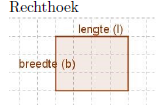
\includegraphics[width=5cm]{4_opp_inhoud_an_meetk/inputs/fig1.png}
		\end{tabular}
		& $O=2(l+b)$ & $A=l.b$ \\
		\begin{tabular}{l}
			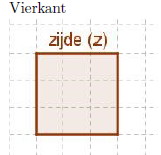
\includegraphics[width=5cm]{4_opp_inhoud_an_meetk/inputs/fig2.png}
		\end{tabular} & $O=4z$ & $A=z^2$ \\
		\begin{tabular}{l}
			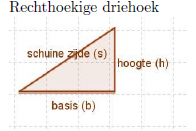
\includegraphics[width=5cm]{4_opp_inhoud_an_meetk/inputs/fig3.png}
		\end{tabular} & $O=b+h+s$ & $A=\frac{b.h}{2}$ \\
		\begin{tabular}{l}
			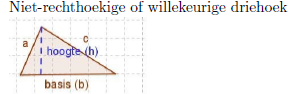
\includegraphics[width=8cm]{4_opp_inhoud_an_meetk/inputs/fig4.png}
		\end{tabular} & $O=a+b+c$ & $A=\frac{b.h}{2}$ 
	\end{tabular}
\end{center}
\caption{Omtrek en oppervlakte van vlakke figuren (1).}
\label{tab:omtrek_opp1}
\end{sidewaystable}
\begin{sidewaystable}
	\begin{center}
		\begin{tabular}{lll}
			Figuur & Omtrek & Oppervlakte \\
			\hline
		\begin{tabular}{l}
			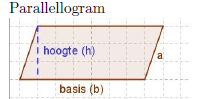
\includegraphics[width=7cm]{4_opp_inhoud_an_meetk/inputs/fig5.png}
		\end{tabular} & $O=2(a+b)$ & $A=b.h$ \\
		\begin{tabular}{l}
			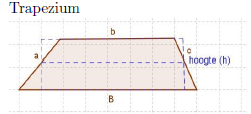
\includegraphics[width=8cm]{4_opp_inhoud_an_meetk/inputs/fig6.png}
		\end{tabular} & $O=a+b+c+B$ & \begin{tabular}{l}
			$A=\frac{b+B}{2}.h$ \\
			Als basis gebruiken we de gemiddelde breedte
		\end{tabular} \\
		\begin{tabular}{l}
			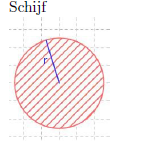
\includegraphics[width=5cm]{4_opp_inhoud_an_meetk/inputs/fig7.png}
		\end{tabular} & \begin{tabular}{l}
			$O=2\pi r$ \\
			Diameter $D=2.r$ \\
			$r$ is de straal
		\end{tabular} &
		\begin{tabular}{l}
			$A=\pi r^2$ \\
			$A=\frac{\pi D^2}{4}$
		\end{tabular} \\
		\begin{tabular}{l}
			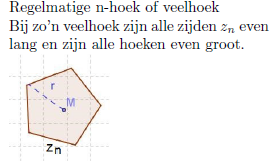
\includegraphics[width=8cm]{4_opp_inhoud_an_meetk/inputs/fig8.png}
		\end{tabular} &
		\begin{tabular}{l}
			$O=n.z_n$ \\
			$O=n.2r.\sin(\frac{\pi}{n})$
		\end{tabular} & $A=n.r^2.\sin(\frac{\pi}{n}).\cos(\frac{\pi}{n})$
	\end{tabular}
\end{center}
\caption{Omtrek en oppervlakte van vlakke figuren (2).}
\label{tab:omtrek_opp2}
\end{sidewaystable}


In de MOOC zie je een animatie die de formule voor de berekening van de oppervlakte van een trapezium verklaart.

\subsection{Ruimtefiguren}

\subsubsection{Prisma}
Een prisma, zie Figuur \ref{fig:ruimtefigurenoppinhoudprisma}, is een ruimtefiguur waarvan twee zijvlakken evenwijdig zijn (bv. het grond- en bovenvlak) en de overige zijvlakken zijn evenwijdig met eenzelfde lijn die de evenwijdige vlakken snijdt. Een prisma wordt dus begrensd door twee evenwijdige en even grote veelhoeken (drie-, vier-, vijfhoeken,... ) die we het \emph{grondvlak en het bovenvlak} noemen. De \emph{opstaande zijvlakken} bestaan uit rechthoeken of parallellogrammen. De ribben die niet in het grond- of bovenvlak gelegen zijn hebben allen dezelfde lengte, we noemen ze de \emph{opstaande ribben}.

Naargelang het aantal opstaande zijvlakken spreken we van een driezijdig, vierzijdig, vijfzijdig,... prisma.

Een \emph{recht} prisma is een prisma, waarin de verbindende ribben en zijvlakken loodrecht op het grondvlak staan. Dit houdt in dat de verbindende zijvlakken rechthoeken zijn. Een scheef \emph{prisma} is een prisma, waarvan de verbindende ribben en zijvlakken niet loodrecht op het grondvlak staan. Dit houdt in dat de verbindende zijvlakken parallellogrammen zijn.

\begin{figure}
	\centering
	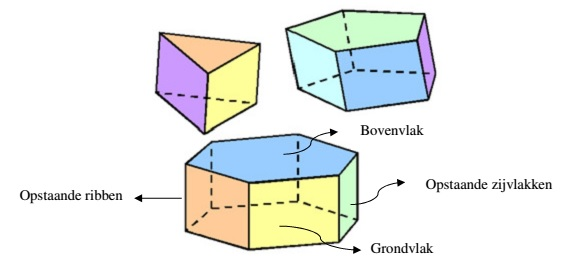
\includegraphics[width=0.7\linewidth]{4_opp_inhoud_an_meetk/inputs/RuimteFigurenOppInhoud_prisma}
	\caption{Prisma.}
	\label{fig:ruimtefigurenoppinhoudprisma}
\end{figure}


\emph{Onthoud}

\fbox{\begin{minipage}{\linewidth}
		
		Oppervlakte van een prisma: $A=\text{opp}_{\text{grondvlak}}+\text{opp}_{\text{bovenvlak}}+\text{opp}_{\text{zijkanten}}$
		
		Volume van een prisma: $V=\text{opp}_{\text{grondvlak}}.\text{hoogte}$
		
	\end{minipage}
}

We onderscheiden een drietal bijzondere prisma's.

\subsubsection{Kubus of hecta\"eder}
Elk zijvlak van de kubus vormt een vierkant, zie Figuur \ref{fig:ruimtefigurenoppinhoudkubus}. Alle 8 ribben zijn dus even lang. Een kubus is een bijzonder recht prisma.

\begin{figure}
	\centering
	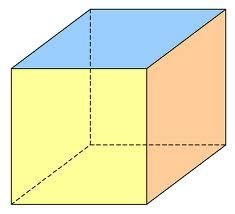
\includegraphics[width=0.7\linewidth]{4_opp_inhoud_an_meetk/inputs/RuimteFigurenOppInhoud_kubus}
	\caption{Kubus}
	\label{fig:ruimtefigurenoppinhoudkubus}
\end{figure}


\emph{Onthoud}

\fbox{\begin{minipage}{\linewidth}
		
		Oppervlakte van een prisma: $A=6z^2$
		
		Volume van een prisma: $V=z^3$
		
	\end{minipage}
}

\subsubsection{Balk}
De 6 zijvlakken van de balk bestaan uit rechthoeken, zie Figuur \ref{fig:ruimtefigurenoppinhoudbalk}. Een balk is ook een bijzonder recht prisma.
Een balk is tevens een rechthoekig parallellepipedum.

\begin{figure}
	\centering
	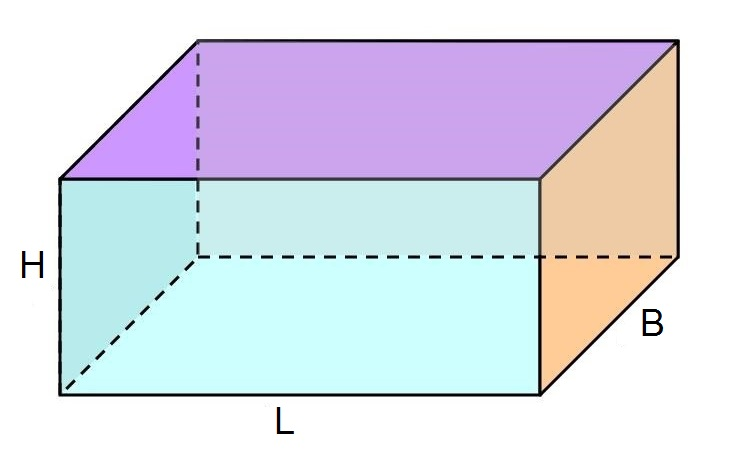
\includegraphics[width=0.7\linewidth]{4_opp_inhoud_an_meetk/inputs/RuimteFigurenOppInhoud_balk}
	\caption{Balk.}
	\label{fig:ruimtefigurenoppinhoudbalk}
\end{figure}


\emph{Onthoud}

\fbox{\begin{minipage}{\linewidth}
		
		Oppervlakte van een prisma: $A=2(L.B+B.H+H.L)$
		
		Volume van een prisma: $V=L.B.H$
		
	\end{minipage}
}


\subsubsection{Parallellepipedum}
Een parallellepipedum, zie Figuur \ref{fig:ruimtefigurenoppinhoudparallellepipedum}, is een veelvlak waarvan alle 6 zijvlakken bestaan uit parallellogrammen die paarsgewijs gelijk en evenwijdig zijn. Dus ook het grond- en het bovenvlak zijn parallellogrammen. Een parallellepipedum is een bijzonder scheef prisma, terwijl de kubus en de balk speciale gevallen zijn van een parallellepipedum.

\begin{figure}
	\centering
	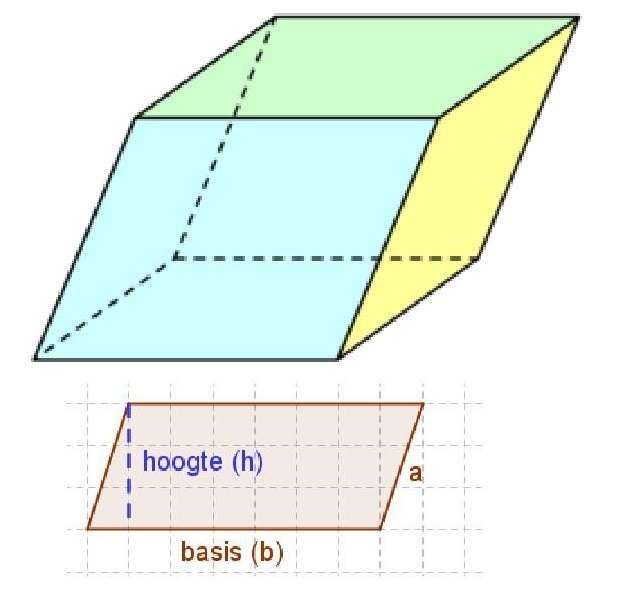
\includegraphics[width=0.7\linewidth]{4_opp_inhoud_an_meetk/inputs/RuimteFigurenOppInhoud_parallellepipedum}
	\caption{Parallellepipedum.}
	\label{fig:ruimtefigurenoppinhoudparallellepipedum}
\end{figure}


\emph{Onthoud}

\fbox{\begin{minipage}{\linewidth}
		
		Oppervlakte van een prisma: $A=\text{som van de oppervlakten}$
		
		Volume van een prisma: $V=\text{opp}_{\text{grondvlak}}.\text{hoogte}$
		
	\end{minipage}
}

\subsubsection{Piramide}
Een piramide is een ruimtefiguur waarvan het grondvlak een veelhoek (driehoek, vierhoek, vijfhoek, $\ldots$) is en waarvan de hoekpunten verbonden worden met een willekeurig punt in de ruimte, zie Figuur \ref{fig:piramide}. Dit punt noemen we de top van de piramide. De opstaande zijvlakken zijn allemaal driehoekig. Een rechte piramide heeft als grondvlak een regelmatige veelhoek en de top ligt boven het centrum van het grondvlak. Alle zijvlakken hebben dezelfde driehoekige vorm.

\begin{figure}
	\centering
	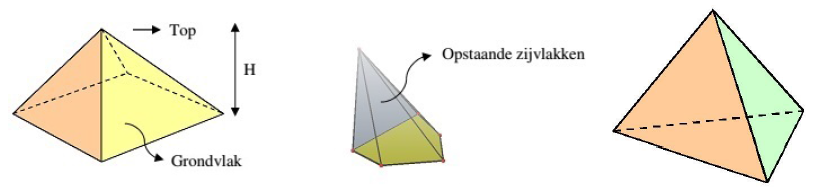
\includegraphics[width=0.7\linewidth]{4_opp_inhoud_an_meetk/inputs/piramide}
	\caption{Piramide.}
	\label{fig:piramide}
\end{figure}


\emph{Onthoud}

\fbox{\begin{minipage}{\linewidth}

Oppervlakte: $A=$ som van alle oppervlakten
\\
Volume: $V=\frac{1}{3}\text{opp}_{\text{grondvlak}}.\text{hoogte}$
\end{minipage}}

Een \emph{tetra\"eder of viervlak} is een ruimtefiguur bestaande uit vier driehoekige vlakken. Het is dus een piramide met een driehoekig grondvlak.

Een \emph{regelmatig viervlak} bestaat uit vier gelijkbenige driehoeken.


\subsection{Omwentelingslichamen}

Deze lichamen hebben ten minste \'e\'en grensvlak dat niet vlak is. We noemen dit vlak een gebogen vlak of zijdelingsoppervlak of manteloppervlak. Omwentelingslichamen ontstaan door het wentelen van een vlak rond een rechte. Deze rechte noemen we dan de omwentelingsas.

\subsubsection{Cilinder}
Een cilinder is een lichaam dat ontstaat wanneer we een rechthoek met afmetingen  $R$ en $H$ om n van zijn zijden laten wentelen, zie Figuur \ref{fig:ruimtefigurenoppinhoudcilinder1}. Beschouw de omwentelingscilinder, met $R$ als de straal van het grond- en bovenvlak en $H$ als de hoogte.

Het grond- en bovenvlak zijn twee evenwijdige schijven met de zelfde straal $R$. De afstand tussen (de middelpunten van) het grond- en bovenvlak noemen we de hoogte $H$. Bij een \emph{rechte cilinder} staat de omwentelingsas loodrecht op het grondvlak, zo niet dan spreken we van een \emph{scheve cilinder}.

De totale oppervlakte van de cilinder is gelijk aan de som van de oppervlakten van het grond- en het bovenvlak (= oppervlakte schijf is $\pi R^2$) en de zijdelingse oppervlakte (= een rechthoek met oppervlakte $2\pi R.H$). De inhoud van de cilinder is het product van oppervlakte grondvlak met de hoogte.

\begin{figure}[h]
	\centering
	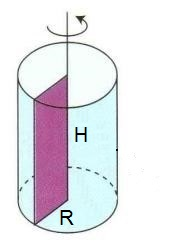
\includegraphics[width=0.3\linewidth]{4_opp_inhoud_an_meetk/inputs/RuimteFigurenOppInhoud_cilinder1}
	\caption{Cilinder}
	\label{fig:ruimtefigurenoppinhoudcilinder1}
\end{figure}

\emph{Onthoud}

\fbox{\begin{minipage}{\linewidth}
		
		Oppervlakte: $A=2\pi R^2 + 2\pi RH$
		\\
		Volume: $V=\pi R^2 H$
\end{minipage}}

\subsubsection{Kegel}
Een kegel is het lichaam dat ontstaat als we een rechthoekige driehoek laten wentelen om \'e\'en van zijn rechthoekszijden, zie Figuur \ref{fig:ruimtefigurenoppinhoudkegel1}. Het grondvlak van de kegel is een schijf met straal $R$. De afstand van de top tot het middelpunt van het grondvlak noemen we de hoogte $H$ van de kegel. Het apothema $a$ van de kegel is de lengte van het lijnstuk $[AB]$, we spreken ook wel van de schuine hoogte. De lengte van het apothema kan gemakkelijk berekend worden a.d.h.v. de stelling van Pythagoras: $a=R+H$.

De totale oppervlakte van de kegel is gelijk aan de som van de oppervlakte van het grondvlak (= oppervlakte schijf is $\pi R^2$) en de zijdelingse oppervlakte ($\pi R a$). De inhoud van de kegel is het product van oppervlakte grondvlak met de hoogte en de constante.

\begin{figure}[h]
	\centering
	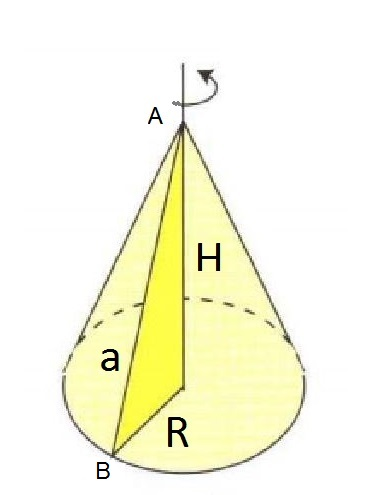
\includegraphics[width=0.3\linewidth]{4_opp_inhoud_an_meetk/inputs/RuimteFigurenOppInhoud_kegel1}
	\caption{Kegel}
	\label{fig:ruimtefigurenoppinhoudkegel1}
\end{figure}


\emph{Onthoud}

\fbox{\begin{minipage}{\linewidth}
		
		Oppervlakte: $A=\pi R^2 + \pi R a$ 
		\\
		Volume: $V=\frac{1}{3}\pi R^2 H$
\end{minipage}}

\subsubsection{Bol}
Een bol is het lichaam dat ontstaat als we een schijf laten wentelen om de middellijn, zie Figuur \ref{fig:ruimtefigurenoppinhoudbol1}. Een bol heeft maar \'e\'en zijvlak, we spreken van het boloppervlak. Alle punten van het boloppervlak liggen op dezelfde afstand van het middelpunt. Deze afstand noemen we de straal $R$.

\begin{figure}[h]
	\centering
	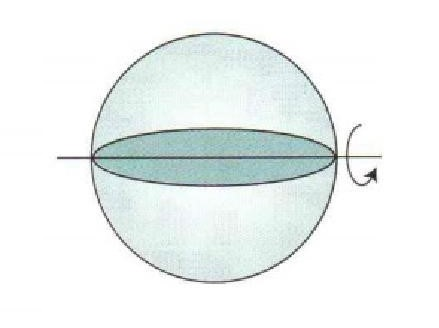
\includegraphics[width=0.3\linewidth]{4_opp_inhoud_an_meetk/inputs/RuimteFigurenOppInhoud_bol1}
	\caption{Bol}
	\label{fig:ruimtefigurenoppinhoudbol1}
\end{figure}


\emph{Onthoud}

\fbox{\begin{minipage}{\linewidth}
		
		Oppervlakte: $A=4\pi R^2$
		\\
		Volume: $V=\frac{4}{3}\pi R^3$
\end{minipage}}


\subsection{Test oppervlakte en inhoudsberekeningen}
TODO

\pagebreak

\section{Analytische meetkunde}

\subsection{Abscis van een punt op een geijkte rechte}

De verzameling $\mathbb{R}$ van de re\"ele getallen kun je voorstellen als de verzameling van de punten op een geijkte rechte.
Een geijkte rechte is een rechte $l$ waarop een paar van 2 verschillende punten $(A;B)$ gekozen is.
De volgorde van zulke punten heeft belang.
Het eerste punt $A$ heet de oorsprong van de ijk.
Deze oorsprong komt overeen met het getal 0.
Het tweede punt $B$ komt overeen met het getal 1.

\gewonefiguur{height=2cm}{4_opp_inhoud_an_meetk/inputs/AMTekst1Fig1}

%\begin{figure}[h]
%\begin{center}
%
\includegraphics[height=2 cm]{4_opp_inhoud_an_meetk/inputs/AMTekst1Fig1}
%\end{center}
%\end{figure}

De richting van $A$ naar $B$ noem je de positieve richting van de geijkte rechte.
Omdat op $l$ door de ijk een positieve richting gedefinieerd is noem je $l$ ook een geori\"enteerde rechte.
Die ori\"entatie duidt je vaak aan met een pijl.
Je stelt een geori\"enteerde rechte ook voor zoals op volgende tekening.

\gewonefiguur{height=2cm}{4_opp_inhoud_an_meetk/inputs/AMTekst1Fig2}

%\begin{figure}[h]
%\begin{center}
%
\includegraphics[height=7 mm]{4_opp_inhoud_an_meetk/inputs/AMTekst1Fig2}
%\end{center}
%\end{figure}

Een natuurlijk getal $n$ (bijvoorbeeld 3) komt overeen met het punt $C$ op $l$ langs dezelfde kant van $A$ als het punt $B$ door $n$ keer vanuit $A$ de afstand van $A$ naar $B$ af te passen.
Je ziet dit ge\"illustreert voor $n=3$.

\gewonefiguur{height=2cm}{4_opp_inhoud_an_meetk/inputs/AMTekst1Fig3}

%\begin{figure}[h]
%\begin{center}
%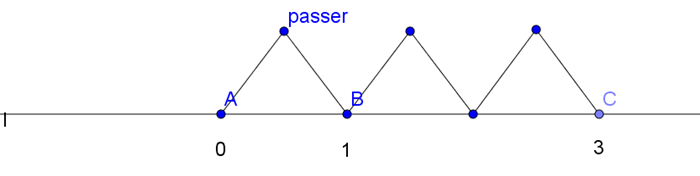
\includegraphics[height=2 cm]{4_opp_inhoud_an_meetk/inputs/AMTekst1Fig3}
%\end{center}
%\end{figure}

%Voor de makers: mijn voorstel is dit uit voor te doen met passer gefilmd door een topcamera.
%Met passer van $A$ naar $B$ afpassen.
%Dit daarna vanuit B naar rechts afpassen (dat geeft op de rechte het niet benoemde punt).
%En van daaruit nog eens naar rechts afpassen (dat geeft dan het punt C). \vspace{5mm}

\subsubsection{Rationaal getal}

Een rationaal getal gegeven door een positieve breuk $\frac{n}{m}$ stel je als volgt voor door een punt $C$ op $l$.
Je verdeelt het lijnstuk van $A$ naar $B$ in $m$ gelijke delen (je ziet straks hoe je dat kunt construeren).
Noem $B'$ het eerste deelpunt na $A$.
Als $n=a+\frac{n'}{m}$ met $0<n'<m$ en $a$ een natuurlijk getal, dan duidt je eerst het punt $C'$ aan op $l$ dat overeenkomt met het natuurlijke getal $a$.
Vervolgens pas je vanuit $C'$ in de positieve richting $n'$ keer de afstand van $A$ naar $B'$ af.
Dit is het punt $C$.

Je ziet dit ge\"illustreerd voor $\frac{n}{m}=\frac{11}{4}=2+\frac{3}{4}$ (dus $a=2$ en $n'=3$).\vspace{5mm}

%Voor de makers: mijn voorstel is ook dit voor te doen met passer en lineaal door een topcamera.
%Je start met de geijkte rechte waar $A$ en $B$ op liggen.
%Je tekent door $A$ de tweede snijdende rechte en kiest daarop een ijk $(A;B_0)$.
%Met de passer pas je op de rechte het punt $Q_0$ af dat met 4 overeen komt. Dat geeft als resultaat de eerste figuur.

%Vervolgens wordt het lijnstuk $Q_0B$ getekend en door met evenwijdig lijnstukken daaraan te werken bekomt men de verdeling van $A$ naar $B$ in 4 gelijke delen.
%(Evenwijdige rechten kun je tekenen door een lineaal en een winkelhaak (rechthoekige driehoek) die je over dat lineaal verschuift)
%Dit geeft dan het punt $B'$ en het resultaat is de tweede figuur.
%
%Tenslotte wordt door het afpassen met de passer (index 1) eerst het punt $C'$ gevonden en daarna door afpassen met de passer (index 2) het punt $C$.

\subsubsection{Negatief getal}

%\begin{figure}[h]
%	\begin{center}
%		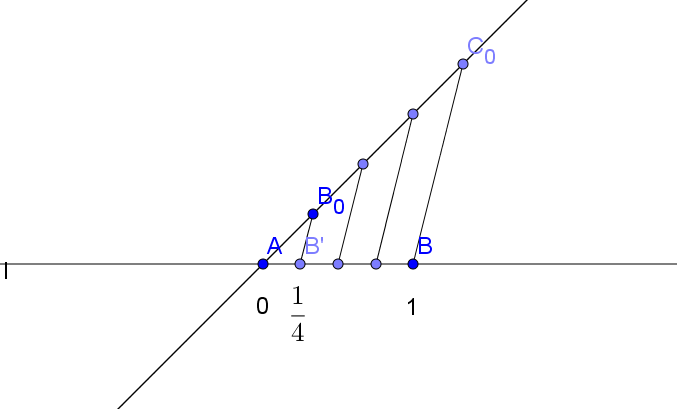
\includegraphics[height=2 cm]{4_opp_inhoud_an_meetk/inputs/AMTekst1Fig5}
%	\end{center}
%\end{figure}
%
%\begin{figure}[h]
%	\begin{center}
%		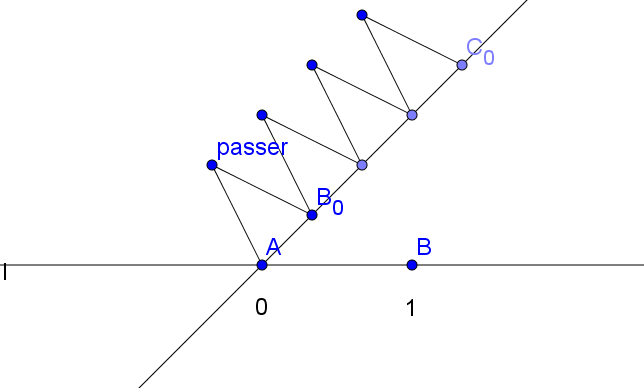
\includegraphics[height=2 cm]{4_opp_inhoud_an_meetk/inputs/AMTekst1Fig4}
%	\end{center}
%\end{figure}

%\begin{figure}[h]
%\begin{center}
%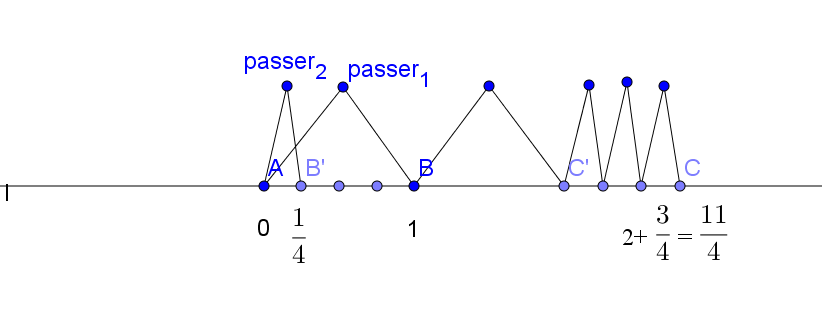
\includegraphics[height=2 cm]{4_opp_inhoud_an_meetk/inputs/AMTekst1Fig6}
%\end{center}
%\end{figure}

Een negatief geheel getal of een negatief rationaal getal construeer je door afstanden af te passen naar de negatieve richting van de geijkte rechte $l$.

\subsubsection{Re\"eel getal}

Met veel meer geavanceerde wiskunde kan aangetoond worden dat ieder re\"eel getal (kommagetal) overeenkomt met een punt van $l$ en dat ieder punt van $l$ ook overeenkomt met een re\"eel getal. Een geijkte rechte is daardoor een meetkundige voorstelling van de verzameling $\mathbb{R}$ van de re\"ele getallen.\vspace{2mm}

Door gebruik te maken van de Stelling van Pythagoras kun je bijvoorbeeld ook het punt van $l$ dat overeenkomt met een vierkantswortels uit een natuurlijk getal construeren.
Je ziet dit ge\"illustreerd voor $\sqrt{5}$.
Je gebruikt daarbij dan $\sqrt{5}$ de schuine zijde is van een rechthoekige driehoek met rechthoekszijden 1 en 2.\vspace{5mm}

%Voorde makers: mijn voorstel is ook dit te voor te doen met passer en lineaal door een topcamera.
Je start met de geijkte rechte waar $A$ en $B$ op liggen.
Loodrecht (winkelhaak) op $l$ door $B$ trek je een rechte en daarop pas je met passer tweemaal vanuit $B$ de afstand van $A$ tot $B$ af.
Dit geeft het punt $B'$ en het resultaat is te zien in Figuur \ref{4.2.1_fig_reeel_fig1}.

Met de passer met middelpunt $A$ en straal de afstand van $A$ tot $B'$ maak je een cirkelboog die op $l$ het punt $C$ geeft.
Het resultaat is te zien in Figuur \ref{4.2.1_fig_reeel_fig2}.

\gewonefiguur{width=.5\linewidth}{4_opp_inhoud_an_meetk/inputs/AMTekst1Fig7}
\gewonefiguur{width=.5\linewidth}{4_opp_inhoud_an_meetk/inputs/AMTekst1Fig8}

%\begin{figure}[h]
%\begin{center}
%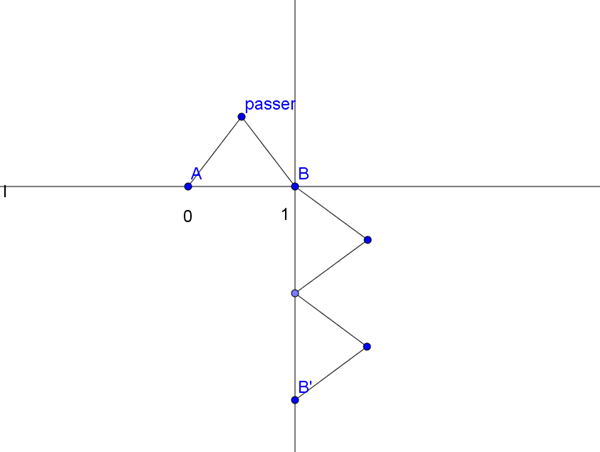
\includegraphics[width=.5\linewidth]{4_opp_inhoud_an_meetk/inputs/AMTekst1Fig7}
%\caption{Constructie vierkantswortel van een natuurlijk getal (1).}
%\label{4.2.1_fig_reeel_fig1}
%\end{center}
%\end{figure}

%\begin{figure}[h]
%\begin{center}
%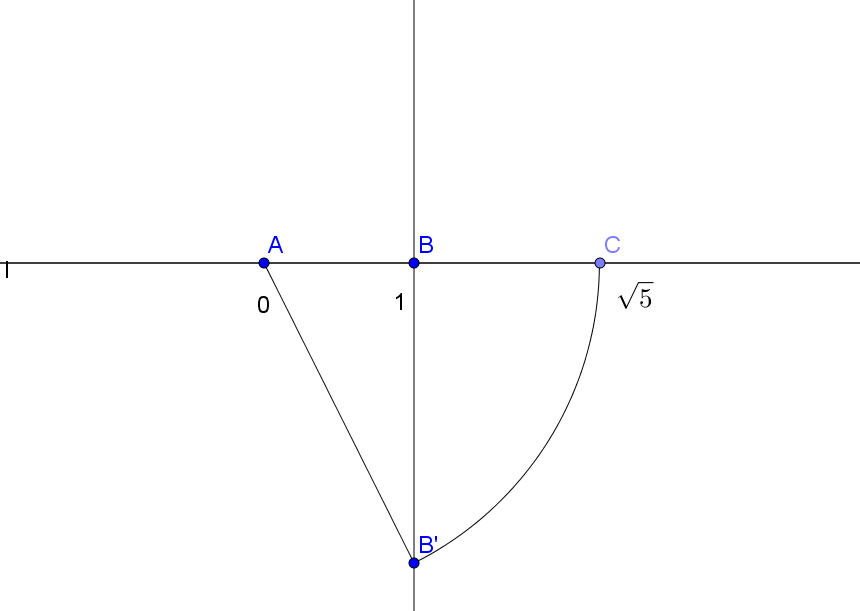
\includegraphics[width=.5\linewidth]{4_opp_inhoud_an_meetk/inputs/AMTekst1Fig8}
%\caption{Constructie vierkantswortel van een natuurlijk getal (2).}
%\label{4.2.1_fig_reeel_fig2}
%\end{center}
%\end{figure}

Algemeen kan voor ieder positief rationaal getal het punt op $l$ dat overeenkomt met de vierkanstwortel geconstrueerd worden.

Wiskundig kan aangetoond worden dat je het punt dat op $l$ overeenkomt met $\sqrt[3]{2}$ niet op soortgelijke wijze kunt construeren.
Ook een re\"eel getal zoals $\pi$ kun je niet op $l$ construeren.\vspace{2mm}

\begin{definitie}
	Voor een punt $P$ op $l$ noem je het re\"ele getal $x$ dat met $P$ overeenkomt de abscis van $P$ en je schrijft $\ab (P)=x$.
\end{definitie}

\gewonefiguur{height=3cm}{4_opp_inhoud_an_meetk/inputs/AMTekst1Fig9}

%\begin{figure}[ht]
%\begin{center}
%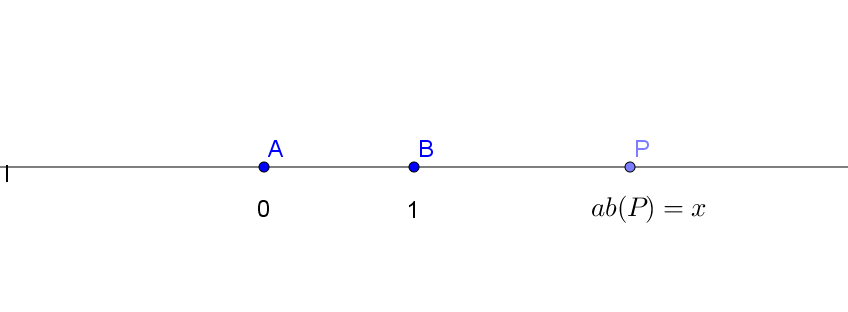
\includegraphics[height=3 cm]{4_opp_inhoud_an_meetk/inputs/AMTekst1Fig9}
%\end{center}
%\end{figure}

Merk op dat je pas over de abscis van een punt op een rechte kunt spreken nadat een ijk op de rechte vastgelegd is.\vspace{2mm}

\begin{voorbeeld}
	
%(Mijn voorstel is om dit voorbeeld uit leggen met lightboard.)
$l$ is een geijkte rechte met ijk $(A;B)$.
$B'$ is het punt op $l$ met $\ab (B')=-\frac{4}{3}$ en $P$ is het punt op $l$ met $\ab (P)=\frac{12}{5}$.
Wat is de abscis van $P$ als je op $l$ de ijk $(A;B')$ neemt?

\gewonefiguur{height=3cm}{4_opp_inhoud_an_meetk/inputs/AMTekst1Fig10}

%\begin{figure}[ht]
%\begin{center}
%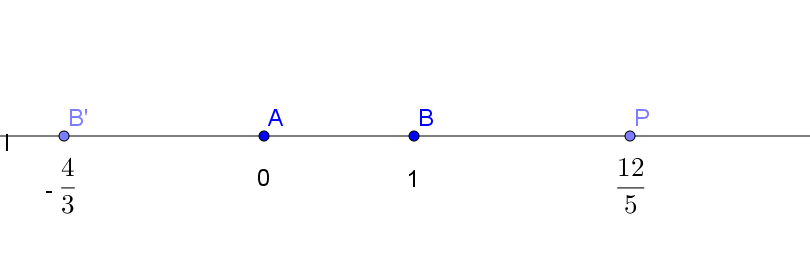
\includegraphics[height=3 cm]{4_opp_inhoud_an_meetk/inputs/AMTekst1Fig10}
%\end{center}
%\end{figure}

Het kleinste gemeenschappelijk veelvoud van 3 en 5 is 15.
Met deze noemer bekom je $\ab (B')=-\frac{20}{15}$ en $\ab (P)=\frac{36}{15}$.
De afstand van $P$ tot $A$ is $\frac{36}{15}.\frac{15}{20}=\frac{36}{20}$-ste van de afstand van $A$ tot $B'$.
Omdat $P$ aan de andere kant van $A$ ligt als $B'$ is de abscis van $P$ ten opzichte van de ijk $(A;B')$ gelijk aan $-\frac{36}{20}=-\frac{9}{5}$.

\end{voorbeeld}
%\begin{figure}[h]
%\begin{center}
%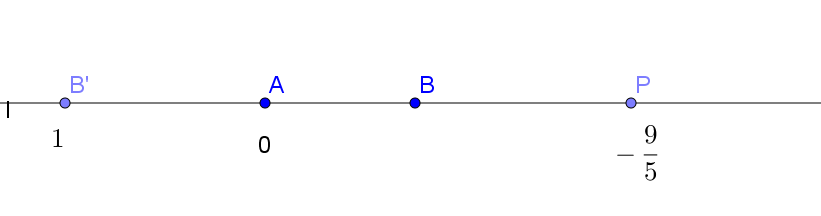
\includegraphics[height=3 cm]{4_opp_inhoud_an_meetk/inputs/AMTekst1Fig11}
%\end{center}
%\end{figure}

\gewonefiguur{height=3cm}{4_opp_inhoud_an_meetk/inputs/AMTekst1Fig11}

Kies een vaste lengte-eenheid (bijvoorbeeld 1 cm) .
Op een rechte $l$ kies je een ijk $(A;B)$ zodat de afstand van $A$ tot $B$ gelijk is aan die lengte-eenheid.
Je zegt dat de geijkte rechte dan overeenkomt met de lengte-eenheid.

Op een geijkte rechte $l$ die overeenkomt met de lengte-eenheid kies je twee punten $P$ en $Q$.
De afstand van $P$ tot $Q$ is dan het verschil tussen de abscissen $\ab (P)$ en $\ab (Q)$.
Noteer $d(P;Q)$ voor de afstand van $P$ tot $Q$.
Je bekomt in dat geval:
\[
d(P;Q)=\vert \ab (Q) - \ab (P) \vert \text { .}
\]



\subsection{Re\"eel getal - voorbeeld} 
Zie filmpje MOOC.

\subsection{Euclidische co\"ordinaten in het vlak}

In het vlak kies je een paar $(l_1;l_2)$ van snijdende rechten met snijpunt $S$, zie Figuur \ref{fig4.2.2_fig1}.
Herinner, bij een paar is de volgorde van belang.
Op beide rechten kies je een ijk met oorsprong $S$.
Op $l_1$ noteer je $(S;B_1)$ voor die ijk en op $l_2$ noteer je $(S;B_2)$.
Zulke twee geijkte rechten in het vlak noem je een assenstelsel in het vlak.
Het snijpunt $S$ van $l_1$ en $l_2$ noem je de oorsprong van het assenstelsel, vaak aangeduid met $O$.

\begin{center}
\tikzsetfigurename{module4_2_3_assenstelsel}
\begin{tikzpicture}
\draw[-] (-2,-0.4)--(5,1) node[anchor=south,left,yshift=0.2cm]{$l_1$};
\draw[-] (-0.4,-2)--(1,5) node[anchor=south,left]{$l_2$};

\tkzDefPoint(0,0){S}
\tkzDefPoint(2,0.4){B1}
\tkzDefPoint(0.4,2){B2}
\tkzDefPoint(3,0.6){P1}
\tkzDefPoint(0.5,2.5){P2}
\tkzDefPoint(3.5,3.1){P}

\tkzLabelPoint[above,xshift=-0.2cm](S){$S$}
\tkzLabelPoint[below](S){$0$}
\tkzLabelPoint[right](S){$0$}

\tkzLabelPoint[above](B1){$B_1$}
\tkzLabelPoint[below](B1){$1$}
\tkzLabelPoint[left](B2){$B_2$}
\tkzLabelPoint[right](B2){$1$}

\tkzLabelPoint[above,xshift=0.3cm](P1){$P_1$}
\tkzLabelPoint[below](P1){$x$}
\tkzLabelPoint[left](P2){$P_2$}
\tkzLabelPoint[right,yshift=0.2cm](P2){$y$}

\tkzLabelPoint[above](P){$P³(x,y)$}

\tkzDrawSegment[black!60!black](P1,P)
\tkzDrawSegment[black!60!black](P2,P)

\foreach \n in {S,B1,B2,P1,P2,P}
\node at (\n)[circle,fill,inner sep=1.5pt]{};
\end{tikzpicture}
\end{center}

%\gewonefiguur{width=\linewidth}{4_opp_inhoud_an_meetk/inputs/AMTekst2Fig1}

%\begin{figure}[!htb]
%\begin{center}
%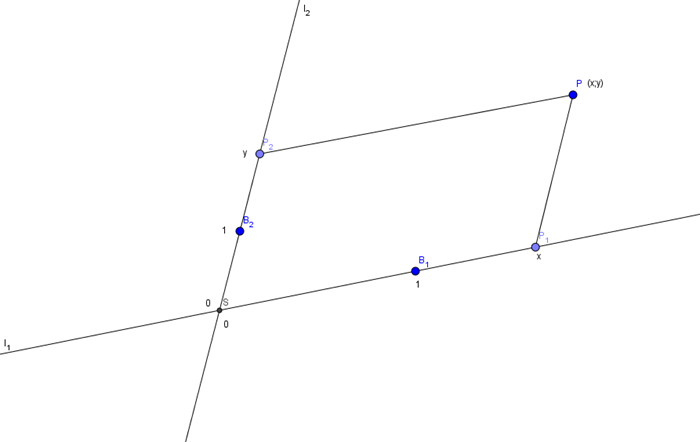
\includegraphics[width=\linewidth]{4_opp_inhoud_an_meetk/inputs/AMTekst2Fig1}
%\caption{}
%\label{fig4.2.2_fig1}
%\end{center}
%\end{figure}

Neem een punt $P$ in het vlak.
Het beeld door $P$ te projecteren evenwijdig aan $l_2$ op $l_1$ noem je $P_1$.
De abscis van $P_1$  op de geijkte rechte $l_1$ is $x$.
Het beeld door $P$ te projecteren evenwijdig aan $l_1$ op $l_2$ noem je $P_2$.
De abscis van $P_2$ op de geijkte rechte $l_2$ is $y$.
Je noemt het paar re\"ele getallen $(x;y)$ de co\"ordinaten van $P$ ten opzichte van het assenstelsel.
Je noteert $\co (P)=(x;y)$.
Ook hier bedoelen we met een paar getallen $(x;y)$ dat de volgorde belang heeft.
In dit geval mogen (en kunnen) de twee getallen $x$ en $y$ gelijk zijn.

Je noemt in deze situatie de geijkte rechte $l_1$ vaak de $x$-as en de geijkte rechte $l_2$ de $y$-as.
Op een tekening noteer je vaak $x$ en $y$ bij die assen en je duidt ook de pijl van de ori\"entatie aan, zoals hieronder.

\begin{center}
\tikzsetfigurename{module4_2_3_assenstelselxy}
\begin{tikzpicture}
\draw[->] (-2,-0.4)--(5,1) node[anchor=south,left,yshift=0.2cm]{$x$};
\draw[->] (-0.4,-2)--(1,5) node[anchor=south,left]{$y$};

\tkzDefPoint(0,0){S}
\tkzDefPoint(2,0.4){B1}
\tkzDefPoint(0.4,2){B2}

\tkzLabelPoint[below](S){$0$}
\tkzLabelPoint[right](S){$0$}

\tkzLabelPoint[below](B1){$1$}
\tkzLabelPoint[right](B2){$1$}

\foreach \n in {S,B1,B2}
\node at (\n)[circle,fill,inner sep=1.5pt]{};
\end{tikzpicture}
\end{center}

%\gewonefiguur{height=5cm}{4_opp_inhoud_an_meetk/inputs/AMTekst2Fig2}

%\begin{figure}[!htb]
%\begin{center}
%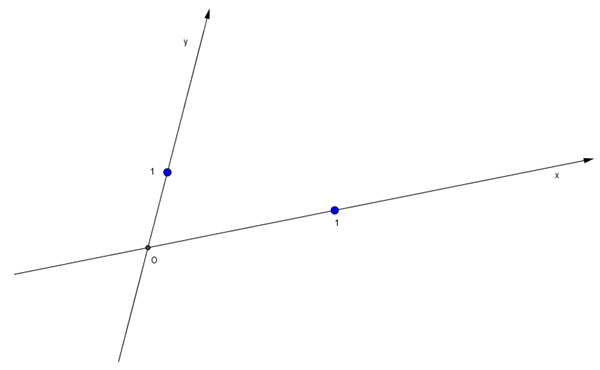
\includegraphics[height=5 cm]{4_opp_inhoud_an_meetk/inputs/AMTekst2Fig2}
%\caption{}
%\label{fig4.2.2_fig2}
%\end{center}
%\end{figure}


\begin{opmerking}
	\begin{itemize}
\item de co\"ordinaten van de oorsprong $O$ zijn $(0;0)$.
\item de co\"ordinaten van punten op de $x$-as zijn van de vorm $(x;0)$.
\item de co\"ordinaten van punten op de $y$-as zijn van de vorm $(0;y)$.
\end{itemize}
\end{opmerking}

Kies een vaste lengte-eenheid (bijvoorbeeld 1 cm).
Een Euclidisch assenstelsel in het vlak is een assenstelsel dat voldoet aan de twee volgende eisen
\begin{itemize}
\item de $x$-as en $y$-as staan loodrecht op elkaar.
\item de geijkte assen $x$ en $y$ komen overeen met de lengte-eenheid.
\end{itemize}
De co\"ordinaten van een punt $P$ in het vlak voorzien van een Euclidisch assenstelsel heten Euclidische co\"ordinaten.
In het vervolg van de cursus (tenzij anders vermeld) gebruiken we enkel Euclidische co\"ordinaten in een vlak.

Vaak teken je een Euclidisch assenstelsel als volgt
\begin{itemize}
\item de $x$-as horizontaal met de positieve richting naar rechts.
\item de $y$-as verticaal met de positieve richting naar boven.
\end{itemize}
In deze ligging is de georiënteerde hoek van de positieve richting van de $x$-as naar de positieve richting van de $y$-as $90^{\circ}$ in tegenwijzerszin, zoals hieronder.
Zulk assenstelsel in het vlak noem je positief geori\"enteerd.


\begin{center}
\tikzsetfigurename{module4_2_3_assenstelselEuclidisch}
\begin{tikzpicture}
\draw[->] (-2,0)--(2,0) node[anchor=south,left,yshift=0.2cm]{$x$};
\draw[->] (0,-2)--(0,2) node[anchor=south,left]{$y$};

\tkzDefPoint(0,0){O}
\tkzDefPoint(0,0){S}
\tkzDefPoint(1,0){A}
\tkzDefPoint(0,1){B}
\tkzDefPoint(-1,0){C}
\tkzDefPoint(3,0){D}
\tkzDefPoint(4,0){E}
\tkzDefPoint(0,-2){F}
\tkzDefPoint(0,-3){G}
\tkzDefPoint(0,4){H}
\tkzDefPoint(0,3){I}
\tkzDefPoint(-1,3){J}
\tkzDefPoint(3,4){K}
\tkzDefPoint(4,-2){L}
\tkzDefPoint(-5,-3){M}
\tkzDefPoint(-5,0){N}

%\tkzDrawSegment[black!60!black,dotted](H,K)
%\tkzDrawSegment[black!60!black,dotted](D,K)
%\tkzDrawSegment[black!60!black,dotted](E,L)
%\tkzDrawSegment[black!60!black,dotted](F,L)	
%\tkzDrawSegment[black!60!black,dotted](G,M)
%\tkzDrawSegment[black!60!black,dotted](N,M)
%\tkzDrawSegment[black!60!black,dotted](C,J)
%\tkzDrawSegment[black!60!black,dotted](I,J)
%
\tkzLabelPoint[below,xshift=-0.2cm](S){$0$}
\tkzLabelPoint[below](A){$1$}
%\tkzLabelPoint[below](D){$3$}
%\tkzLabelPoint[above](E){$4$}
%\tkzLabelPoint[below](C){$-1$}
%\tkzLabelPoint[above](N){$-5$}
\tkzLabelPoint[left](B){$1$}
%\tkzLabelPoint[right](I){$3$}
%\tkzLabelPoint[left](H){$4$}
%\tkzLabelPoint[left](F){$-2$}
%\tkzLabelPoint[right](G){$-3$}
%
%\tkzLabelPoint[left](M){$T$}
%\tkzLabelPoint[above](J){$Q$}
%\tkzLabelPoint[above](K){$P$}
%\tkzLabelPoint[below](L){$R$}

\foreach \n in {A,B,O}
\node at (\n)[circle,fill,inner sep=1.5pt]{};

\pic [draw, ->, "", angle eccentricity=0.5] {angle = A--O--B};

\end{tikzpicture}	
\end{center}


%\gewonefiguur{height=5cm}{4_opp_inhoud_an_meetk/inputs/AMTekst2Fig3}

%\begin{figure}[!htb]
%\begin{center}
%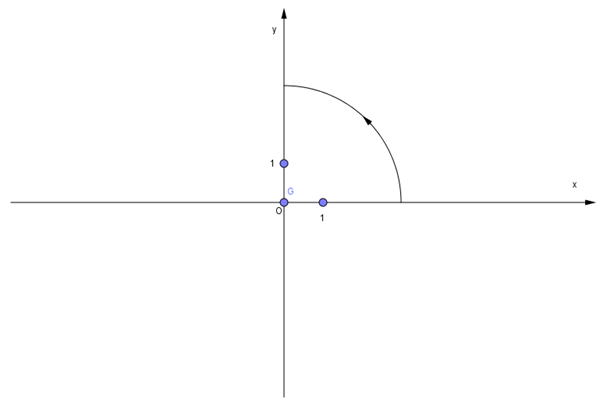
\includegraphics[height=5 cm]{4_opp_inhoud_an_meetk/inputs/AMTekst2Fig3}
%\caption{}
%\label{fig4.2.2_fig3}
%\end{center}
%\end{figure}

Op de volgende figuur zijn in een Euclidisch assenstelsel met die ligging de volgende punten met hun co\"ordinaten aangeduidt: $P(3;4)$, $Q(-1;3)$, $R(4;-2)$ en $T(-5;-3)$.


%\gewonefiguur{width=.7\linewidth}{4_opp_inhoud_an_meetk/inputs/AMTekst2Fig4}

%\begin{figure}[!htb]
%\begin{center}
%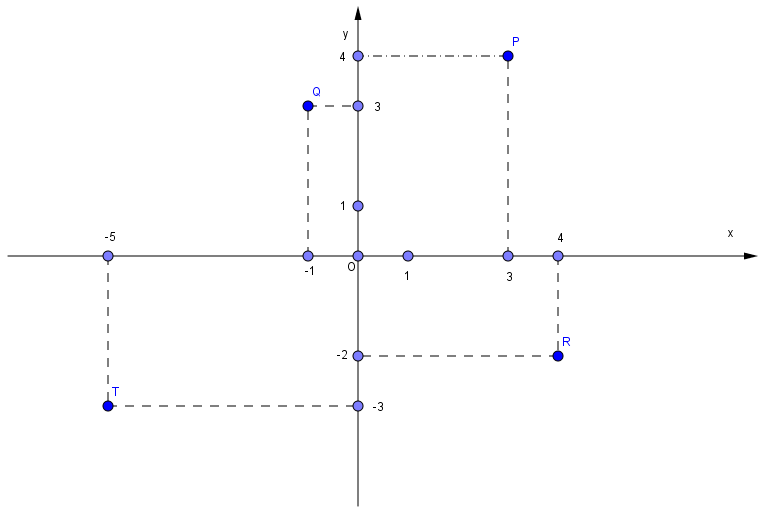
\includegraphics[width=.7\linewidth]{4_opp_inhoud_an_meetk/inputs/AMTekst2Fig4}
%\caption{}
%\label{fig4.2.2_fig4}
%\end{center}
%\end{figure}

Een assenstelsel verdeelt het vlak in 4 delen.
Je noemt dat de kwadranten.
Deze nummer je in tegenwijzerszin. 
Je start met het deel waar $x$ en $y$ allebei positief zijn.
Dat noem je het eerste kwadrant, zoals in de figuur hieronder.

\begin{minipage}{.5\linewidth}
%\gewonefiguur{width=.5\linewidth}{4_opp_inhoud_an_meetk/inputs/AMTekst2Fig5}
\begin{center}
\begin{tabular}{c|c|c}
	Kwadrant & $x$ & $y$ \\
	\hline
	I & + & + \\
	II & - & + \\
	III & - & - \\
	IV & + & - \\
\end{tabular}	
\end{center}
\end{minipage}
\begin{minipage}{.5\linewidth}
\begin{center}
	\tikzsetfigurename{module4_2_3_kwadranten}
\begin{tikzpicture}
\coordinate (a) at (0,0);
\coordinate (b) at (2,0);
\coordinate (c) at (0,2);

\draw[->] (-3,0)--(3,0) node[anchor=south,left,yshift=0.2cm]{$x$};
\draw[->] (0,-3)--(0,3) node[anchor=south,left]{$y$};

\tkzDefPoint(0,0){S}
\tkzDefPoint(1,0){B1}
\tkzDefPoint(0,1){B2}

\tkzLabelPoint[below,xshift=-0.1cm](S){$0$}
\tkzLabelPoint[right,yshift=0.1cm](S){$0$}

\tkzLabelPoint[below](B1){$1$}
\tkzLabelPoint[right](B2){$1$}

\foreach \n in {S,B1,B2}
\node at (\n)[circle,fill,inner sep=1.5pt]{};

%	\node[draw,align=right] at (1,2) {Kwadrant I};
%	\node[draw,align=left] at (-1,2) {Kwadrant II};
%	\node[draw,align=left] at (-1,-1) {Kwadrant III};
%	\node[draw,align=right] at (1,-1) {Kwadrant IV};

\node[] at (1.5,1.5) {Kwadrant I};
\node[] at (-1.5,1.5) {Kwadrant II};
\node[] at (-1.5,-1.5) {Kwadrant III};
\node[] at (1.5,-1.5) {Kwadrant IV};

\end{tikzpicture}	
\end{center}
\end{minipage}


\subsection{Afstand tussen twee punten in het vlak}
\noindent

Het vlak is voorzien van een Euclidisch assenstelsel.
Neem twee verschillende punten $P(a;b)$ en $Q(c;d)$ in het vlak.
We stellen de formule op waarmee je de afstand tussen $P$ en $Q$ (genoteerd $d(P;Q)$ uitdrukt met de Euclidische co\"ordinaten van $P$ en $Q$.

De loodrechte projecties van $P$ en $Q$ op de $x$-as noem je $P_1$ en $Q_1$.
De loodrechte projecties van $P$ en $Q$ op de $y$-as noem je $P_2$ en $Q_2$.
Deze punten hebben co\"ordinaten $P_1(a;0)$, $Q_1(c;0)$, $P_2(0;b)$ en $Q_2(0;d)$.

Als $b=d$ dan is de rechte $PQ$ evenwijdig met de $x$-as.
Als $a=c$ dan is de rechte $PQ$ evenwijdig met de $y$-as.
Stel dat de rechte $PQ$ noch horizontaal, noch verticaal is (dus $b\neq d$ en $a \neq c$).
Het snijpunt van de rechte door $P$ evenwijdig met de $y$-as met de rechte door $Q$ evenwijdig met de $x$-as noem je $R$.

\gewonefiguur{height=5cm}{4_opp_inhoud_an_meetk/inputs/AMTekst3Fig1}

%\begin{figure}[!htb]
%\begin{center}
%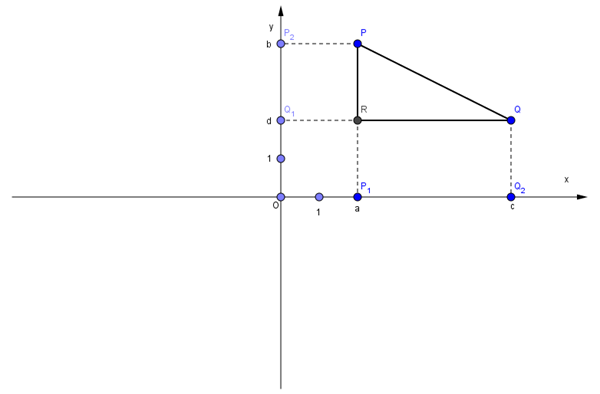
\includegraphics[width=.7\linewidth]{4_opp_inhoud_an_meetk/inputs/AMTekst3Fig1}
%\caption{}
%\label{fig4.2.3_fig1}
%\end{center}
%\end{figure}

In de rechthoekige driehoek $PQR$ geeft de Stelling van Pythagoras:
\[
\vert PQ \vert ^2= \vert PR \vert ^2+ \vert QR \vert ^2 \text {.}
\]
Er geldt $\vert PR \vert = \vert Q_2P_2 \vert = d(Q_2;P_2)=\vert b-d \vert$.
Dit laatste is waar omdat $b$ en $d$ abscissen zijn van $P_2$ en $Q_2$ op de geijkte $y$-as die overeenkomt met de lengte-eenheid.
Er geldt ook $\vert QR \vert = \vert P_1Q_1 \vert = d(P_1;Q_1)=\vert a-c \vert$.
Invullen in de Stelling van Pythagoras geeft
\[
\vert PQ \vert ^2=(b-d)^2+(a-c)^2 \text{ .}
\]
Hieruit vind je
\[
d(P;Q)=\sqrt{(b-d)^2+(a-c)^2} \text { .}
\]\vspace{2mm}

De formule geldt ook als de rechte $PQ$ wel evenwijdig is met de $x$-as of de $y$-as.
\begin{itemize}
\item De rechte $PQ$ is horizontaal, dus $b=d$.

\gewonefiguur{width=.7\linewidth}{4_opp_inhoud_an_meetk/inputs/AMTekst3Fig2}

%\begin{figure}[!htb]
%\begin{center}
%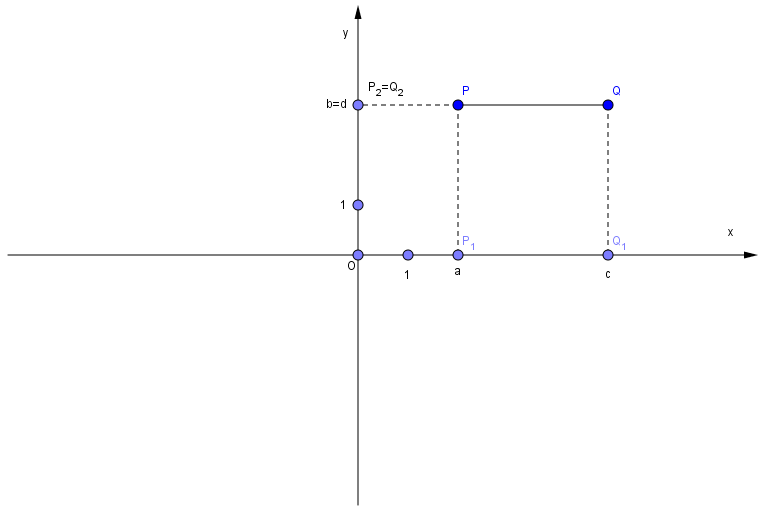
\includegraphics[width=.7\linewidth]{4_opp_inhoud_an_meetk/inputs/AMTekst3Fig2}
%\caption{}
%\label{fig4.2.3_fig2}
%\end{center}
%\end{figure}

\[
d(P;Q)=d(P_1;Q_1)=\vert c-a \vert \text { en } \sqrt { (b-d)^2+(a-c)^2 }=\vert c-a \vert
\]
\item De rechte $PQ$ is verticaal, dus $a=c$.
\gewonefiguur{height=5cm}{4_opp_inhoud_an_meetk/inputs/AMTekst3Fig3}
%\begin{figure}[!htb]
%\begin{center}
%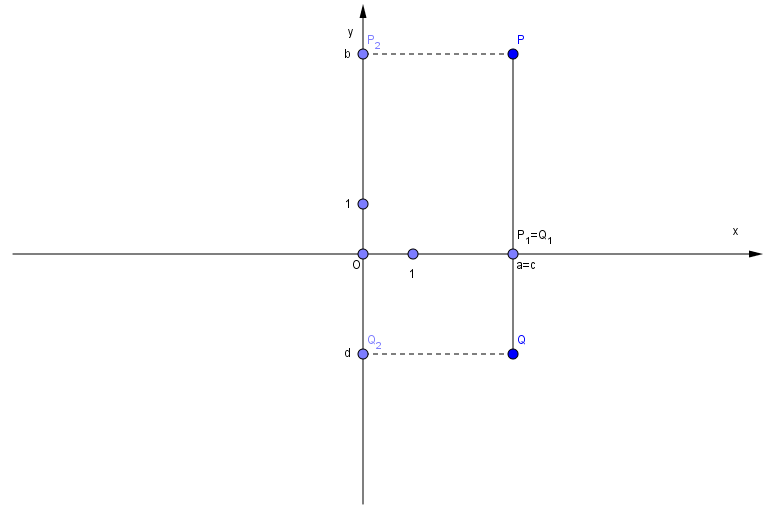
\includegraphics[width=.7\linewidth]{4_opp_inhoud_an_meetk/inputs/AMTekst3Fig3}
%\caption{}
%\label{fig4.2.3_fig3}
%\end{center}
%\end{figure}
\[
d(P;Q)=d(P_2;Q_2)=\vert d-b \vert \text { en } \sqrt { (b-d)^2+(a-c)^2 }=\vert b-d \vert
\]
\end{itemize}\vspace{2mm}

\newpage

\begin{voorbeeld}
Bereken de afstand tussen $P(2;-3)$ en $Q(-5;-2)$.

\gewonefiguur{height=5cm}{4_opp_inhoud_an_meetk/inputs/AMTekst3Fig4}

%\begin{figure}[!htb]
%\begin{center}
%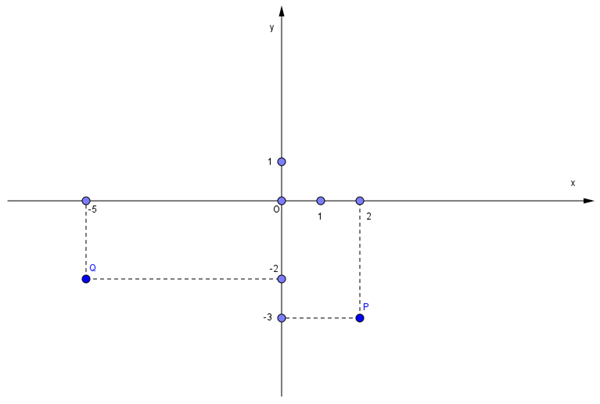
\includegraphics[width=.7\linewidth]{4_opp_inhoud_an_meetk/inputs/AMTekst3Fig4}
%\caption{Voorbeeld 1.}
%\label{fig4.2.3_fig4}
%\end{center}
%\end{figure}
\[
d(P;Q)=\sqrt{(-5-2)^2+(-2-(-3))^2}=\sqrt{50}
\]\vspace{3mm}

%Voor de makers: volgend voorbeeld tekening tonen en daarnaast berekeningen met topcamera.
\end{voorbeeld}

\begin{voorbeeld}
Gegeven zijn de punten $P(-2;5)$ en $Q(3;-1)$.
Wat zijn de co\"ordinaten van het punt $R$ met $x$-co\"ordinaat gelijk aan 2 dat even ver van $P$ als van $Q$ ligt?

\gewonefiguur{height=5cm}{4_opp_inhoud_an_meetk/inputs/AMTekst3Fig5}
%\begin{figure}[!htb]
%\begin{center}
%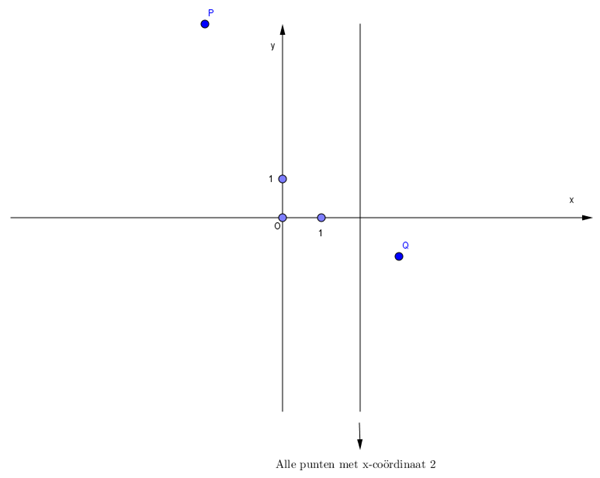
\includegraphics[width=.7\linewidth]{4_opp_inhoud_an_meetk/inputs/AMTekst3Fig5}
%\caption{Voorbeeld 2.}
%\label{fig4.2.3_fig5}
%\end{center}
%\end{figure}

$R$ heeft co\"ordinaten $(2;y)$.
We zoeken $y$ zodat $d(R;P)=d(R;Q)$.
\[
d(R;P)=\sqrt{(-2-2)^2+(y-5)^2}=\sqrt{16+(y-5)^2}
\]
\[
d(R;Q)=\sqrt{(3-2)^2+(y-(-1))^2}=\sqrt{1+(y+1)^2}
\]
Hieruit volgt dat $d(R;P)=d(R;Q)$ als en alleen als
\[
16+(y-5)^2=1+(y+1)^2
\]
Uitwerken van de kwadraten geeft
\[
16+y^2-10y+25=1+y^2+2y+1 \text { dus } 12y=39 \text { .}
\]
Het punt $R$ heeft co\"ordinaten $(2;\frac{39}{12})$.
\end{voorbeeld}

\subsection{Afstand tussen twee punten - voorbeeld} 
Zie filmpje MOOC.

\subsection{Vergelijking van een rechte}
\noindent

Het vlak is voorzien van een Euclidisch assenstelsel met oorsprong $O$.
In het vlak is $l$ een rechte door $O$ verschillend van \'e\'en van de assen van het assenstelsel.
Je neemt op $l$ twee verschillende punten $Q(x_1;y_1)$ en $R(x_2;y_2)$ allebei verschillend van $O$.
Je noemt $Q_1$ (resp.$R_1$) de loodrechte projectie van $Q$ (resp. $R$) op de $x$-as.
Omdat de rechthoekige driehoeken $OQQ_1$ en $ORR_1$ even grote overeenkomstige hoeken hebben zijn ze gelijkvormig.
\begin{figure}[!htb]
\begin{center}
\includegraphics[height=5 cm]{4_opp_inhoud_an_meetk/inputs/AMTekst4Fig1}
\end{center}
\end{figure} 
Hieruit volgt dat de verhoudingen van lengten van overeenkomstige zijden gelijk zijn, dus
\[
\frac {\vert RR_1 \vert}{\vert QQ_1 \vert}=\frac {\vert OR_1 \vert}{\vert OQ_1 \vert} \text { .}
\]
In termen van co\"ordinaten bekom je
\[
\frac {\vert y_1 \vert}{\vert y_2 \vert}=\frac {\vert x_1 \vert}{\vert x_2 \vert} \text { en dus } \frac {\vert y_1 \vert}{\vert x_1 \vert}=\frac {\vert y_2 \vert}{\vert x_2 \vert} \text { .}
\]
Merk op dat op de linkse figuur voor een punt $P(x;y)$ op $l$ verschillende van $O$ steeds geldt dat $\frac {y}{x}>0$ terwijl op de rechtse figuur steeds geldt $\frac {y}{x}<0$.
De tekens van $\frac {y_1}{x_1}$ en $\frac {y_2}{x_2}$ zijn dus steeds gelijk en je bekomt daardoor zelfs
\[
\frac {y_1}{x_1} = \frac{y_2}{x_2} \text { .}
\]
Je bekomt hieruit dat een getal $m \in \mathbb{R}_0$ bestaat zodat voor ieder punt $P(x;y)$ op $l$ verschillende van $O$ geldt
\[
\frac {y}{x}=m \text { en dus } y=mx \text { .}
\]
Deze laatste vergelijking is een nodige en voldoende voorwaarde opdat een punt $P(x;y)$ in het vlak tot de rechte $l$ behoort.
Het is een vergelijking van $l$.
Voor $l$ als op de linkse figuur is $m>0$ en voor $l$ als op de rechtse figuur is $m<0$.

Als $l$ de $x$-as is dan behoort een punt $P(x;y)$ van het vlak tot $l$ als en alleen als $y=0$.
Dit laatste is dan een vergelijking van $l$ (dus van de $x$-as).
Merk op, door $m=0$ te nemen in vorig resultaat bekom je dat je de vergelijking eveneens in de vorm $y=0.x$ kan schrijven.

Als $l$ de $y$-as is dan behoort een punt $P(x;y)$ van het vlak tot $l$ als en alleen als $x=0$.
Dit laatste is dan een vergelijking van $l$ (dus van de $y$-as).
Merk op, er is geen enkel getal $m$ zodat je die laatste vergelijking kunt schrijven in de vorm $y=mx$.

Voor een rechte $l$ door de oorsprong is $\alpha$ een geori\"enteerde hoek van de $x$-as naar $l$.
\begin{itemize}
\item Een geori\"enteerde hoek is positief in tegenwijzerszin en negatief in wijzerszin.
\item De hoek $\alpha$ is slechts op een veelvoud van $180^o$ ($\pi$ radialen) na bepaald (zie de figuur).
\end{itemize}
\begin{figure}[!htb]
\begin{center}
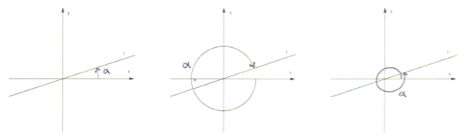
\includegraphics[height=4 cm]{4_opp_inhoud_an_meetk/inputs/AMtekst4Fig2}
\end{center}
\end{figure}
Zulke geori\"enteerde hoek komt overeen met een punt op de goniometrische cirkel.
Uit de constructie van de tangens bekom je dat $(1; \tan \alpha)$ de co\"ordinaten zijn van een punt op $l$ (als $l$ niet de $y$-as is).
Omdat de punten van $l$ moeten voldoen aan een vergelijking $y=mx$ bekom je $m=\tan \alpha$.

Samengevat bekomen we het volgende resultaat.
De vergelijking van een rechte $l$ door de oorsprong $O$ verschillend van de $y$-as is $y=(\tan \alpha )x$.
Hierbij is $\alpha$ de geori\"enteerde hoek tussen de positieve $x$-as en de rechte $l$.
De vergelijking van de $y$-as is $x=0$.\\

Een rechte $l$ die niet door de oorsprong $O$ gaat en niet evenwijdig is met de $y$-as snijdt de $y$-as in een punt $Q(0;q)$.
De rechte $l'$ door de oorsprong $O$ die evenwijdig is aan $l$ heeft een vergelijking $y=mx$.

Voor een punt $P(x;y)$ op $l$ is $P'$ de projectie van $P$ op $l$ evenwijdig met de $y$-as.
\begin{figure}[!htb]
\begin{center}
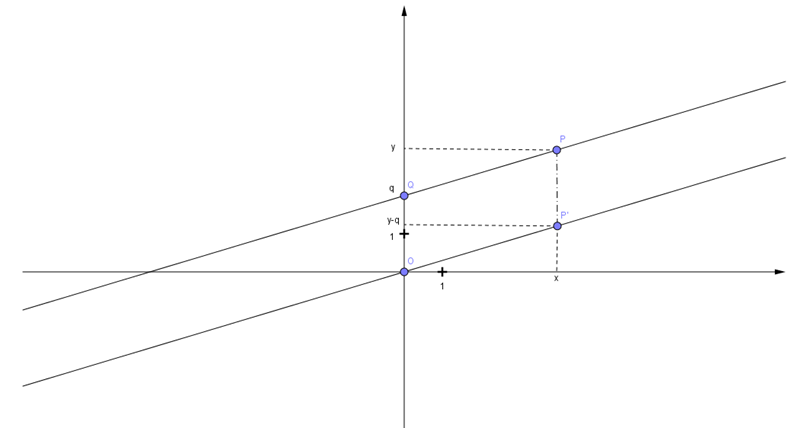
\includegraphics[height=8 cm]{4_opp_inhoud_an_meetk/inputs/AMtekst4Fig3}
\end{center}
\end{figure} 
De co\"ordinaten van $P'$ zijn $(x;y-q)$ en omdat $P'$ tot de rechte $l'$ met vergelijking $y=mx$ behoort moet $y-q=mx$.
Je bekomt dat een nodige en voldoende voorwaarde opdat een $P(x;y)$ in het vlak tot de rechte $l$ behoort is $y=mx+q$.
Dat getal $m$ is $\tan \alpha$ met $\alpha$ de geori\"enteerde hoek tussen de positieve $x$-as en de rechte $l$.
Je noemt $m$ de richtinsco\"effici\"ent van $l$ en je noteert $m=\rico (l)$.

Je besluit : een vergelijking van $l$ is $y=mx+q$.

Indien $l$ een rechte is evenwijdig met de $y$-as dan bestaat $a \in \mathbb{R}$ zodat $l$ bestaat uit alle punten $P(x;y)$ in het vlak waarvoor $x=a$.
In dat geval in $x=a$ een vergelijking van $l$.
Merk op dat je zulke vergelijking niet kunt schrijven in vorm $y=mx+q$, zulke rechte $l$ heeft geen richtingsco\"effici\"ent.

\noindent \underline{Opmerking:} Als $\rico(l)=m$ en $P_0(x_0;y_0)$ is een punt op $l$ dan is
\[
y-y_0=m(x-x_0)
\]
een vergelijing van $l$.
Duidelijk voldoen de co\"ordinaten van $P_0$ aan de vergelijking.
Je kunt de vergelijking herleiden tot de vorm $y=mx+(y_0-mx_0)$.
Dit is van de vorm $y=mx+q$ met $q=y_0-mx_0$ en dus de vergelijking van een rechte.
In die laatste vorm herken je ook dat $m$ de richtinsco\"effici\"ent is van die rechte.\\

%Aan de makers van de cursus: ik stel voor hier een filmpje toe te voegen.Dit filmpje moet de invloed van $l$ en $m$ op de ligging van de rechte met vergelijking $y=mx+q$ illustreren.
%Wat nu volgt is een voorstel voor het scenario van dat filmpje.
%
%\noindent \underline{Fimpje}
%
%$y=mx$ tekenen waarbij $m$ van -3 naar 3 toeneemt (toename van $m$ met vaste snelheid; als mogelijk op voorhand vermelden wat gaat gebeuren (met geluid dus) en daarbij vermelden dat de richting zelf het snelste verandert als de rico dicht bij 0 is).
%
%$y=2x+q$ tekenen waarbij $q$ van -3 naar 3 toeneemt. Ook snijpunt met de $y$-as duidelijk erbij tekenen (toename van $q$ opnieuw met constante snelheid, op voorhand vertellen wat gaat gebeuren en opmerken dat ook het snijpunt met de $y$-as met constante snelheid zal bewegen).
%
%$y-1=-\frac {1}{2} (x-a)$ tekenen waarbij $a$ van -3 naar 3 toeneemt. Ook het punt met $y$-co\"ordinaat 1 erbij tekenen (toename van $a$ opnieuw met constante snelheid, op voorhand vertellen wat gaat gebeuren en opmerken dat ook het punt met $y$-co\"ordinaat gelijk aan 1 met constante snelheid zal bewegen).
%
%Hiermee be\"eindigt dan het filmpje.\\

%Aan de makers van de cursus : mijn voorstel is om het volgende voorbeeld met topcamera te maken.

\subsection{Vergelijking rechte - voorbeeld}
Zie filmpje MOOC.

\subsection{Vergelijking rechte met richting en door gegeven punt - extra voorbeelden}
Zie filmpje MOOC.

\subsection{Vergelijking rechte met richting en door gegeven punt - extra voorbeelden}

\noindent \underline{Voorbeeld 1:} Geef een vergelijking van de rechte $l$ zodat de geori\"enteerde hoek tussen de positieve $x$-as en $l$ gelijk is aan $30^o$ en zodat het punt $P(2;-5)$ tot  $l$ behoort, zie Figuur \ref{fig4.2.9_fig4}.
Geef eveneens de co\"ordinaten van het snijpunt van $l$ met de $x$-as en met de $y$-as.

\begin{figure}[!htb]
\begin{center}
\includegraphics[height=5 cm]{4_opp_inhoud_an_meetk/inputs/AMTekst4Fig4}
\caption{Voorbeeld 1.}
\label{fig4.2.9_fig4}
\end{center}
\end{figure} 

Er geldt $\rico (l)=\tan (30^o)=\frac {1}{\sqrt{3}}$.
De vergelijking van $l$ is $y-(-5)=\frac{1}{\sqrt{3}}(x-2)$ en je bekomt
\[
y=\frac{1}{\sqrt{3}}x-5-\frac{2}{5} \text { dus } y=0,577x-6,155 \text { .}
\]
Omdat $q=-6,155$ is heeft het snijpunt $A$ met de $y$-as co\"ordinaten $(0;-6,155)$.
(Dit vind je ook door $x=0$ in de vergelijking in te vullen.)
Op de $x$-as is $y=0$. Voor het snijpunt $B$ met de $x$-as geldt daarom $0,577x-6,155=0$.
Je bekomt
\[
x=\frac{6,155}{0,577}=10,667 \text { .}
\]
Het snijpunt $B$ met de $x$-as heeft co\"ordinaten $(10,667;0)$.\\

We stellen nu de vergelijking op van een rechte door twee gegeven verschillende punten $P_1(x_1;y_1)$ en $P_2(x_2;y_2)$.
Als $x_1=x_2$ dan is de rechte evenwijdig met de $y$-as en de vergelijking is $x=a$ (met $a=x_1$).

Stel dat $x_1 \neq x_2$ (de rechte is dus niet evenwijdig met de $y$-as).
De rechte heeft een vergelijking van de vorm $y=mx+q$.
Deze vergelijking moet gelden als je de co\"ordinaten van $P_1$ en $P_2$ invult.
Dit geeft volgende gelijkheden:
\[
y_1=m.x_1+q \text { en } y_2=m.x_2+q \text { .}
\]
Neem je van beide leden van deze twee gelijkheden telkens het verschil dan bekom je
\[
y_2-y_1=m.(x_2-x_1) 
\]
en omdat $x_1 \neq x_2$ bekom je
\[
\rico (P_1P_2)=m=\frac {y_2-y_1}{x_2-x_1} \text { .}
\]
Je bekomt als vergelijking van de rechte $P_1P_2$
\[
y-y_1=\frac {y_2-y_1}{x_2-x_1} (x-x_1) \text { .}
\]\\

\noindent \underline{Voorbeeld:} Geef een vergelijking van de rechte $l$ door de punten $P(3;5)$ en $Q(-2;4)$, zie Figuur \ref{fig4.2.9_fig5}.

\begin{figure}[!htb]
\begin{center}
\includegraphics[height=5 cm]{4_opp_inhoud_an_meetk/inputs/AMTekst4Fig5}
\caption{Voorbeeld 1.}
\label{fig4.2.9_fig5}
\end{center}
\end{figure}

Invullen in voorgaande formule geeft
\[
y-5=\frac{4-5}{-2-3}(x-3)
\]
en mits wat rekenwerk bekom je hieruit
\[
y=\frac{1}{5}x+\frac{22}{5} \text { .}
\]\\

Je kunt een vergelijking van een rechte steeds schrijven in de vorm $ax+by+c=0$ met $a$ en $b$ niet allebei 0.
Omgekeerd, een vergelijking van de vorm $ax+by+c=0$ met $a$ en $b$ niet allebei gelijk aan 0 steeds een vergelijking van een rechte.
\begin{itemize}
\item Indien $b=0$ dan is $a \neq 0$ en je kunt de vergelijking omvormen tot $x=-\frac{c}{a}$.
Je bekomt een rechte evenwijdig met de $y$-as (door het punt $(-\frac{c}{a};0)$).
\item Indien $b \neq 0$ dan kun je de vergelijking omvormen tot
\[
y=\left( -\frac{a}{b}  \right)x+\left(  -\frac{c}{b} \right) \text { .}
\]
Je bekomt de rechte met richtingsco\"effici\"ent $-\frac {a}{b}$ door het punt $(0; -\frac{c}{b})$.
\end{itemize}


\subsection{Onderlinge ligging van twee rechten}
\noindent

Twee rechten $l_1$ en $l_2$ in het vlak zijn evenwijdig als en alleen als de positieve richting van de $x$-as even grote geori\"enteerde hoeken maakt met $l_1$ en met $l_2$.
Hieruit volgen twee mogelijkheden:
\begin{itemize}
\item $l_1$ en $l_2$ zijn allebei evenwijdig met de $y$-as.
\item $\rico (l_1)=\rico (l_2)$ (en dan zijn $l_1$ en $l_2$ niet evenwijdig met de $y$-as).
\end{itemize}

%Aan de makers: mijn voorstel is volgend voorbeeld te maken met een topcamera.


\begin{voorbeeld}
Gegeven zijn 3 punten $A(2:-3)$, $B(-1;4)$ en $C(3;4)$.
Geef een vergelijking van de rechte $l$ door $C$ evenwijdig aan de rechte $AB$.

\gewonefiguur{height=7cm}{4_opp_inhoud_an_meetk/inputs/AMTekst5Fig1}

%\begin{figure}[!htb]
%\begin{center}
%\includegraphics[height=7 cm]{4_opp_inhoud_an_meetk/inputs/AMTekst5Fig1}
%\caption{Voorbeeld 1.}
%\label{fig4.2.10_fig1}
%\end{center}
%\end{figure} 
De richtingsco\"effici\"ent $m$ van rechte $AB$ is
\[
m=\frac {4-(-3)}{-1-2}=-\frac {7}{3} \text { .}
\]
De richtingsc\"effici\"ent van $l$ moet dus ook -4 zijn.
Omdat $l$ ook door het punt $C$ moet gaan bekomen we volgende vergelijking van $l$:
\[
y-4=(-\frac {7}{3})(x-3) \text { dus } 7x+3y-33=0 \text { .}
\]\\

Een loodlijn op een rechte evenwijdig met de $x$-as (vergelijking van de vorm $y=b$) is een rechte evenwijdig met de $y$-as (vergelijking van de vorm $x=a$).
\end{voorbeeld}

\begin{voorbeeld}
	$l$ is de rechte met vergelijking $y=5$.
Geef een vergelijking van de loodlijn $l'$ op $l$ door $P(3;-4)$.

\gewonefiguur{height=7cm}{4_opp_inhoud_an_meetk/inputs/AMTekst5Fig2}

%\begin{figure}[!htb]
%\begin{center}
%\includegraphics[height=7 cm]{4_opp_inhoud_an_meetk/inputs/AMTekst5Fig2}
%\caption{Voorbeeld 2}
%\label{fig4.2.10_fig2}
%\end{center}
%\end{figure} 
Omdat $l'$ een rechte is evenwijdig met de $y$-as heeft $l'$ een vergelijking van de vorm $x=a$.
Omdat $(P3;-4)$ op $l'$ moet liggen moet $a=3$.
Een vergelijking van $l'$ is dus $x=3$.

Een loodlijn op een rechte evenwijdig met de $y$-as (vergelijking van de vorm $x=a$) is een rechte evenwijdig met de $x$-as (vergelijking van de vorm $y=b$).

Stel nu dat $l$ aan geen van beide assen evenwijdig is.
Stel dat $\alpha$ een ge\"ori\"enteerde hoek is tussen de positieve richting van de $x$-as en de rechte $l$.
In dat geval is de grootte van de hoek $\alpha$ geen veelvoud van $90^o$.
Dit impliceert dat de richtingsco\"effici\"ent $m=\tan (\alpha$ van de rechte $l$ bestaat en verschillend is van 0.
Als $l'$ een loodlijn is op $l$ dan is $\alpha + 90^o$ een geori\"enteerde hoek tussen de positieve richting van de $x$-as en $l'$.
Omdat $\tan (\alpha + 90^o)=-\cot (\alpha)=-\frac{1}{\tan (\alpha)}$  bekom je dat $\rico (l')=-\frac{1}{m}=-\frac{1}{\rico (l)}$.

\underline {Besluit:} Als $l$ en $l'$ loodrechte op elkaar staan en geen van beide is evenwijdig met een as van het assenstelsel dan is
\[
\rico (l).\rico (l')=-1 \text { .}
\]

\end{voorbeeld}
%Aan de makers: mijn voorstel is volgend voorbeeld te maken met een topcamera.


\begin{voorbeeld}
	Gegeven zijn de rechte $l$ met vergelijking $y=2x-3$ en het punt $P(-2;3)$.
Geef een vergelijking voor de loodlijn $l'$ door $P$ op $l$.
Geef eveneens de co\"ordinaten van de loodrechte projectie van $P$ op $l$.

\gewonefiguur{height=7cm}{4_opp_inhoud_an_meetk/inputs/AMTekst5Fig3}

%\begin{figure}[!htb]
%\begin{center}
%\includegraphics[height=7 cm]{4_opp_inhoud_an_meetk/inputs/AMTekst5Fig3}
%\caption{Voorbeeld 3}
%\label{fig4.2.10_fig3}
%\end{center}
%\end{figure} 

Omdat $\rico (l)=2$ is $\rico (l')=-\frac{1}{2}$.
Omdat $l'$ ook door $P(-3;2)$ moet gaan is de vergelijking van $l'$
\[
y-3=-\frac{1}{2}(x+2) \text { dus } y=-\frac{1}{2}+2 \text { .}
\]

De loodrechte projectie van $P$ op $l$ is het snijpunt $P'$ van de rechten $l$ en $l'$.
De co\"ordinaten $(x,y)$ van het punt $P'$ moeten dus voldoen aan de vergelijkingen van beide rechten:
\[
l \leftrightarrow y=2x-3 \text { en } l' \leftrightarrow y=-\frac{1}{2}x+2 \text { .}
\]
Voor de $x$-co\"ordinaat van $P'$ bekom je hieruit de vergelijking
\[
2x-3=-\frac{1}{2}x+2
\]
met als oplossing $x=2$.
Vul je dit in de vergelijking van $l$ (of $l'$) in dan bekom je de $y$-co\"ordinaat van $P'$:
\[
y=2.2-3=1 \text { .}
\]
De co\"ordinaten van $P'$ zijn $(2;1)$.\\

Twee verschillende punten $A$ en $B$ in het vlak bepalen een lijnstuk $[AB]$.
De middelloodlijn van dat lijnstuk $[AB]$ is de rechte $l$ loodrecht op de rechte $AB$ door het midden $M$ van het lijnstuk $[AB]$.
Deze middelloodlijn is eveneens de verzameling van alle punten $P$ in het vlak die evenver van $A$ als van $B$ liggen.
In volgend voorbeeld zie je dit nagerekend.\\

\end{voorbeeld}

\begin{voorbeeld}
Gegeven zijn de punten $A(3;4)$ en $B(-2;1)$.
\begin{itemize}
\item We berekenen eerst een vergelijking van de middelloodlijn $l$ op $[AB]$ door de definitie te gebruiken.
Het midden $M$ van het lijnstuk $[AB]$ is het punt waarvan de co\"ordinaten de gemiddelden zijn van de co\"ordinaten van $A$ en $B$, dus 
\[
M(\frac{3+(-2)}{2};\frac{4+1}{2})=(\frac{1}{2};\frac{5}{2}) \text { .}
\]
De richtingsco\"effici\"ent van de rechte $AB$ is $\rico (AB)=\frac {1-4}{-2-3}=\frac{3}{5}$.
De richtingsco\"effici\"ent van de middelloodlijn $l$ is dus $\rico (l)=-\frac{5}{3}$.
Je bekomt daardoor als vergelijking van de rechte $l$:
\[
y-\frac{5}{2}=-\frac{5}{3}(x-\frac{1}{2}) \text { dus } y=-\frac{5}{3}x+\frac{10}{3} \text { .}
\]
\item We stellen nu een vergelijking op voor de verzameling van de punten $P$ in het vlak die evenver van $A$ als van $B$ liggen.
Een punt $P(x,y)$ ligt evenver van $A$ als van $B$ als en alleen als
\[
\sqrt{(x-3)^2+(y-4)^2}=\sqrt{(x+2)^2+(y-1)^2} \text { .}
\]
Kwadrateren van beide positieve leden in voorgaande gelijkheid en uitrekenen van de kwadraten geeft volgende nodige en voldoende voorwaarde
\[
x^2-6x+9+y^2-8y+16=x^2+4x+4+y^2-2y+1 \text { .}
\]
Merk op dat de kwadraten verdwijnen en als je alles oplost naar de veranderlijke $y$ dan bekom je
\[
y=-\frac{5}{3}x+\frac{10}{3} \text { .}
\]
\end{itemize}
Je merkt op dat je in beide delen dezelfde vergelijking bekomt.
In dit voorbeeld bekomen we dus dat de verzameling van de punten $P$ evenver gelegen van $A$ en $B$ hetzelfde is als de middelloodlijn op het lijnstuk $[AB]$.
Dit kan met behulp van elementaire meetkunde in alle gevallen bewezen worden (dat doen we in deze cursus niet).\\

\end{voorbeeld}

Gegeven zijn twee rechten $l$ en $l'$ met vergelijkingen
\[
l \leftrightarrow ax+by+c=0 \text { en } l' \leftrightarrow a'x+b'y+c'=0 \text { .}
\]
Hoe vind je de scherpe hoek $\angle (l,l')$ tussen de rechten $l$ en $l'$?

Uit de vergelijkingen kun je direct zien of een rechte evenwijdig is met de $y$-as.
Van een rechte die niet evenwijdig is met de $y$-as kun je de richtingsco\"effici\"ent uit de vergelijking vinden.
De richtingsco\"effici\"ent (als deze bestaat) van $l$ duiden we aan met $m$ en van $l'$ met $m'$.
Met deze richtingsco\"effici\"enten bereken je dan de geori\"enteerde hoek $\alpha$ (resp $\alpha '$) tussen de positieve richting van de $x$-as en de rechte $l$ (resp. $l'$) en genomen met grootte in het interval $]-90^o;90^o]$ (voor een verticale rechte nemen we dus $90^o$).

Door eventueel $l$ en $l'$ te verwisselen kunnen we aannemen dat $\alpha \geq \alpha '$.
Dan is $\angle (l,l')$ gelijk aan $\alpha - \alpha '$ als dit hoogstens $90^o$ is en anders is $\angle (l,l')$ gelijk aan $180^o-(\alpha - \alpha ')$.
Als $l$ evenwijdig is met de $y$-as dan bekomen we dat $\angle (l,l')=90^o-\vert \alpha \vert$.
We veronderstellen nu dat $l$ niet evenwijdig is met de $y$-as (en $l'$ dus ook niet).

Uit de vergelijkingen bekom je
\[
\rico (l)=m=-\frac {a}{b} \text { en dus } \tan (\alpha )=m=-\frac{a}{b}
\]
\[
\rico (l')=m'=-\frac{a'}{b'} \text { en dus } \tan(\alpha ')=m'=-\frac{a'}{b'}
\]
Omdat $\tan (\alpha -\alpha ')=\frac{\tan (\alpha)-\tan (\alpha ')}{1+\tan (\alpha).\tan (\alpha ')}$; $\tan (180^o-(\alpha -\alpha '))=-\tan (\alpha -\alpha ')$ en de tangens van een scherpe hoek steeds positief is bekom je
\[
\tan (\angle (l,l'))=\vert \frac{m-m'}{1+m.m'} \vert
\]
(als $1+m.m'=0$ dan staan $l$ en $l'$ loodrecht op elkaar) of nog
\[
\tan (\angle (l,l'))=\vert \frac{-\frac{a}{b}-(-\frac{a'}{b'})}{1+(-\frac{a}{b})-\frac{a'}{b'}} \vert = \vert \frac{a'b-ab'}{aa'+bb'} \vert \text { .}
\]
Vanwege de absolute waarden is het niet meer nodig dat in deze formules $\alpha \geq \alpha$.\\


%\noindent \underline{Voorbeeld 1:} Gegeven zijn de punten $A(3;-2)$, $B(-4;1$ en $C(1;3)$.
%Bereken de scherpe hoek tussen de rechten $BA$ en $BC$.
%\begin{figure}[!htb]
%\begin{center}
%\includegraphics[height=7 cm]{4_opp_inhoud_an_meetk/inputs/AMTekst5Fig5}
%\end{center}
%\end{figure} 
%Je berekent eerst de richtingsco\"effici\"enten van de rechten $AB$ en $BC$.
%\[
%\rico (BC)=m=\frac{3-1}{1-(-4)}=\frac{2}{5}
%\]
%\[
%\rico (BA)=m'=\frac{1-(-2)}{-4-3}=-\frac{3}{7}
%\]
%Invullen in de formule met richtingsco\"effici\"enten geeft
%\[
%\tan (\angle (BC;BA) )=\frac{m-m'}{1+m.m'}=\frac{\frac{2}{5}-(-\frac{3}{7})}{1+(\frac{2}{5}).(-\frac{3}{7})}=1 \text { .}
%\]
%Je bekomt $\angle (BC;BA) = \arctan (1)=45^o$.\\
%
%Voorstel aan de makers is volgend voorbeeld als een lightboard filmpje toe te voegen.\\
%
%\noindent \underline{Voorbeeld 2:} Gegeven is de rechte $l$ met vergelijking $6x-3y+2=0$ en $P(-1;2)$.
%Stel een vergelijking op voor iedere rechte $l'$ door $P$ waarvoor $\angle (l.l')=30^o$.
%
%Er geldt $\rico (l)=m=2$.
%We noteren $\rico (l')=m'$.
%We moeten bekomen dat $\tan (\angle (l,l'))=\tan (30^o)=\frac {\sqrt {3}}{3}$.
%We gaan de formule gebruiken waarbij $\tan (\angle (l,l'))$ wordt uitgedrukt met de richtingsco\"effici\"enten van $l$ en $l'$.
%Omdat de hoek van $30^o$ tussen $l$ en $l'$ in twee richtingen kan voorkomen bekomen we twee mogelijke vergelijkingen om $m'$ uit te vinden:
%\[
%\frac {\sqrt{3}}{3}=\frac {m-m'}{1+m.m'}=\frac{2-m'}{1+2m'}
%\]
%\[
%\frac {\sqrt{3}}{3}=\frac {m'-m}{1+m.m'}=\frac {m'-2}{1+2m'} \text { .}
%\]
%De eerste vergelijking geeft
%\[
%(1+2m')\sqrt {3}=3(2-m') \text { waaruit } m'=\frac {6-\sqrt{3}}{3+2\sqrt {3}}=0,66 \text { .}
%\]
%De vergelijking van de bijbehorende rechte $l'$ is
%\[
%y-2=0,66(x+1) \text { dus } y=0,66x+2,66 \text { .}
%\]
%De tweede vergelijking geeft
%\[
%(1+2m')\sqrt {3}=3(m'-2) \text { waaruit } m'=\frac {-6+-\sqrt {3}}{2 \sqrt {3}-3}=-16,66 \text { .}
%\]
%De vergelijking van de bijbehorende rechte $l'$ is
%\[
%y-2=-16,66(x+1) \text { dus } y=-16,66x-14,66 \text { .}
%\]
%


\subsection{Onderlinge ligging van twee rechten - voorbeeld 1}
Zie filmpje MOOC.

\subsection{Onderlinge ligging van twee rechten - voorbeeld 2}
Zie filmpje MOOC.

\subsection{Onderlinge ligging van twee rechten - voorbeeld 3}
Zie filmpje MOOC.

\subsection{Afstand van een punt tot een rechte}
\noindent

De afstand $d(P;l)$ van een punt $P$ tot een rechte $l$ is de afstand van $P$ tot de loodrechte projectie $P'$ van $P$ op $l$.\\

\begin{voorbeeld}
	Gegeven zijn een punt $P(2;-4)$ en de rechte $l$ met vergelijking $2x-5y+7=0$.
De rechte $l'=PP'$ zal loodrecht staan op $l$.
Omdat $\rico (l)=\frac {2}{5}$ moet $\rico (l')=-\frac {5}{2}$.
De vergelijking van de rechte $PP'=l'$ is daarom
\[
y-(-4)=-\frac {5}{2} (x-2) \text { dus } y=-\frac {5}{2}x+1 \text { .}
\]
Het punt $P'$ is het snijpunt van $l$ en $l'$.
De co\"ordinaten van $P'$ zijn daarom de oplossing van het stelsel
\[
\begin{cases}
y=\frac {2}{5} x +\frac {7}{5} \\
y=-\frac {5}{2} x +1
\end{cases}
\] 
De $x$-co\"ordinaat van $P'$ is daardoor de oplossing van
\[
\frac {2}{5} x+\frac {7}{5} = -\frac {5}{2} x +1 \text { dus } x=-\frac {4}{29} \text { .}
\]
Door deze waarde van $x$ in te vullen in $y=-\frac {5}{2}+1$ (vergelijking van $l'$) bekom je de $y$-co\"ordinaat van $P'$.
\[
y=-\frac {5}{2}.(-\frac{4}{29})+1=\frac {39}{29}
\]
De co\"ordinaten van $P'$ zijn $(-\frac {4}{29}; \frac {39}{29 })$.

De afstand van $P$ tot de rechte $l$ is de afstand van $P$ tot $P'$.
Je bekomt als afstand
\[
\sqrt { \left( 2+\frac {4}{29}  \right)^2 + \left( -4-\frac {39}{29}  \right)^2  } =\frac {\sqrt { 62^2+155^2}}{29}=5,76 \text { .}
\]\\

Er is een heel eenvoudige formule waarmee je de afstand van een punt $P(x_0;y_0)$ tot een rechte $l$ met vergelijking $ax+by+c=0$ kunt uitrekenen.
Je hoeft dan de vorige werkwijze in het voorbeeld niet telkens uit te voeren.
Deze formule is
\[
d(P;l)=\frac { \vert ax_0+by_0+c \vert }{\sqrt {a^2+b^2}} \text { .}
\]\\

Pas je voorgaande formule toe op het voorbeeld dan bekom je
\[
d(P;l)=\frac { \vert 2.2-5.(-4)+7 \vert }{\sqrt {4+25}}=\frac {31}{\sqrt {29}}=5,76 \text { .}
\]
Je merkt dat je inderdaad dezelfde uitkomst bekomt.\\
\end{voorbeeld}

\begin{voorbeeld}
	Gegeven zijn de punten $A(-5;2)$, $B(-1;4)$ en $C(3;-2)$.
Bereken de oppervlakte van driehoek $ABC$.

\begin{center}
	\begin{tikzpicture}
	\draw[->] (-5,0)--(5,0) node[anchor=south,left,yshift=0.2cm]{$x$};
	\draw[->] (0,-4)--(0,6) node[anchor=south,left]{$y$};
	
	\tkzDefPoint(0,0){S}
	\tkzDefPoint(1,0){x1}
	\tkzDefPoint(0,1){y1}
	
	\tkzDefPoint(-5,0){A1}
	\tkzDefPoint(0,2){A2}
	
	\tkzDefPoint(-5,2){A}
	
	\tkzDefPoint(-1,0){B1}
	\tkzDefPoint(0,4){B2}
	
	\tkzDefPoint(-1,4){B}
	
	\tkzDefPoint(3,0){C1}
	\tkzDefPoint(0,-2){C2}
	
	\tkzDefPoint(3,-2){C}
	
	\tkzLabelPoint[below,xshift=-0.1cm](S){$0$}
	%	\tkzLabelPoint[right,yshift=-0.3cm](S){$O$}
	
	\tkzLabelPoint[below](x1){$1$}
	\tkzLabelPoint[left](y1){$1$}
	
	\tkzLabelPoint[left,yshift=0.2cm](A){$A$}
	\tkzLabelPoint[right,yshift=0.2cm](B){$B$}
	\tkzLabelPoint[right,yshift=0.2cm](C){$C$}
			
	\tkzLabelPoint[below](A1){$-5$}
	\tkzLabelPoint[right](A2){$2$}

	\tkzLabelPoint[below](B1){$-1$}
	\tkzLabelPoint[right](B2){$4$}

	\tkzLabelPoint[above](C1){$3$}
	\tkzLabelPoint[left](C2){$-2$}	
	
	\tkzDrawSegment[black!60!black,dotted](A1,A)
	\tkzDrawSegment[black!60!black,dotted](A2,A)
	\tkzDrawSegment[black!60!black,dotted](B1,B)
	\tkzDrawSegment[black!60!black,dotted](B2,B)
	\tkzDrawSegment[black!60!black,dotted](C1,C)
	\tkzDrawSegment[black!60!black,dotted](C2,C)
	
	\tkzDrawSegment[black!60!black](A,C)
	\tkzDrawSegment[black!60!black](A,B)
	\tkzDrawSegment[black!60!black](B,C)
	
	\foreach \n in {S,x1,y1,A1,A2,A,B1,B2,B,C1,C2,C}
	\node at (\n)[circle,fill,inner sep=1.5pt]{};
	
	\end{tikzpicture}
\end{center}

%\gewonefiguur{height=7cm}{4_opp_inhoud_an_meetk/inputs/AMTekst6Fig1}

%\begin{figure}[h]
%\begin{center}
%\includegraphics[height=7 cm]{4_opp_inhoud_an_meetk/inputs/AMTekst6Fig1}
%\caption{Voorbeeld 2.}
%\label{fig4.2.14_fig1}
%\end{center}
%\end{figure} 

We vatten het lijnstuk $[A;B]$ op als basis van de driehoek.
Dan is $d(A;B)$ de lengte van de basis.
De hoogte van de driehoek is dan de afstand $d(C;AB)$ van het punt $C$ tot de rechte $AB$.
Je bekomt
\[
d(A;B)=\sqrt { (-1-(-5))^2+(4-2)^2}=\sqrt {20} \text { .}
\]
Een vergelijking van de rechte $AB$ is
\[
y-2=\frac {4-2}{-1-(-5)}(x-(-5)) \text { dus } 2y-x-9=0 \text { .}
\]
De afstand van $C$ tot de rechte $AB$ is dan
\[
d(C;AB)=\frac {\vert 2.(-2)-3-9 \vert}{\sqrt{4+1}}=\frac {16}{\sqrt {5}} \text { .}
\]
De oppervlakte van driehoek $ABC$ is dus gelijk aan
\[
\frac {d(A;B).d(C;AB)}{2}=\frac { \sqrt {20}.\frac {16}{\sqrt {5}}}{2}=16 \text { .}
\]\\

De bissectrices van twee niet evenwijdige rechten $l$ en $l'$ zijn de rechten die een hoek tussen $l$ en $l'$ in twee gelijke delen verdelen.
Twee niet evenwijdige lijnen $l$ en $l'$ hebben twee bissectrices $b$ en $b'$ die loodrecht op elkaar staan.

\begin{center}
	\begin{tikzpicture}
	\clip (-5,-5) rectangle (5,5);
	
%	\draw[->] (-5,0)--(5,0) node[anchor=south,left,yshift=0.2cm]{$x$};
%	\draw[->] (0,-5)--(0,5) node[anchor=south,left]{$y$};
	
	\draw[domain=-5:5,smooth,variable=\x] plot ({\x},{2/5*\x+4/5}) node[anchor=south,left,yshift=0.2cm] {$l$};	
	\draw[domain=-1:2,smooth,variable=\x] plot ({\x},{-3*\x+2}) node[anchor=south,left,yshift=0.2cm] {$l'$};	
	\draw[domain=-5:5,smooth,variable=\x] plot ({\x},{-9.83/21.2*\x+23.42/21.20}) node[anchor=south,left,yshift=-0.4cm] {$b$};	
	\draw[domain=-3:2,smooth,variable=\x] plot ({\x},{22.48/10.43*\x+1.88/10.43}) node[anchor=south,left,yshift=0.2cm] {$b'$};	
	
	\end{tikzpicture}
\end{center}


%\gewonefiguur{height=7cm}{4_opp_inhoud_an_meetk/inputs/AMTekst6Fig1}

%\begin{figure}[h]
%\begin{center}
%\includegraphics[height=7 cm]{4_opp_inhoud_an_meetk/inputs/AMTekst6Fig2}
%\caption{Bisectrice.}
%\label{fig4.2.14_fig2}
%\end{center}
%\end{figure} 

Er kan aangetoond worden dat deze twee rechten $b$ en $b'$ samen de verzameling is van alle punten $P$ in het vlak die evenver van de rechten $l$ en $l'$ liggen.
Door middel van de formule voor de afstand van een punt tot een rechte kun je met die formule vergelijkingen voor die bissectrices vinden.\\
\end{voorbeeld}

\begin{voorbeeld}
	Stel vergelijkingen op van de bissectrices van de rechten $l$ en $l'$ gegeven door de volgende vergelijkingen.
\[
l \leftrightarrow 2x-5y+4=0 \text { en } l' \leftrightarrow3x+y-2=0 
\]
Een punt $P(x;y)$ behoort tot \'e\'en van de bissectrices $b$ en $b'$ als en alleen als $d(P;l)=d(P;l')$.
Omdat
\[
d(P;l)=\frac { \vert 2x-5y+4 \vert }{\sqrt {4 + 25}} \text { en } d(P;l')=\frac { \vert 3x+y-2 \vert }{\sqrt {9+1}}
\]
bekom je dat $P$ op een bissectrice ligt als en alleen als
\[
\frac { \vert 2x-5y+4 \vert }{\sqrt {29}}=\frac { \vert 3x+y-2 \vert }{\sqrt {10}} \text { .}
\]
Laat je hierin de absolute waarde weg dan zijn de uitdrukkingen aan weerszijden van de gelijkheid gelijk of tegengesteld.
Dit geeft aanleiding tot vergelijkingen van twee rechten: de bissectrices $b$ en $b'$.
Deze vergelijkingen zijn:
\begin{itemize}
\item  voor $b$
\[
\frac {2x-5y+4}{\sqrt {29}}=\frac {3x+y-2}{\sqrt {10 }}
\]
\[
(2\sqrt {10}-3\sqrt {29})x+(-5\sqrt {10}-\sqrt {29})y+(4\sqrt {10}+2\sqrt {29})=0
\]
\[
-9,83x-21,20y+23,42=0
\]
\item voor $b'$
\[
\frac {2x-5y+4}{\sqrt {29}}=-\frac {3x+y-2}{\sqrt {10}}
\]
\[
(2\sqrt {10}+3\sqrt {29})x+(-5\sqrt{10}+\sqrt{29})y+(4\sqrt{10}-2\sqrt{29})=0
\]
\end{itemize}
\[
22,48x-10,43y+1,88=0 \text { .}
\]

\end{voorbeeld}


\subsection{Vergelijking van een cirkel in het vlak}
\noindent

\begin{definitie}
	De cirkel met middelpunt $M(x_0;y_0)$ en straal $r$ ($r>0$) is de verzameling van de punten $P$ in het vlak die op dezelfde afstand $r$ van het middelpunt $M$ liggen.
\end{definitie}

\begin{notatie}
	$C(M,r)$
\end{notatie}

\gewonefiguur{height=7cm}{4_opp_inhoud_an_meetk/inputs/AMTekst7Fig1}

%\begin{figure}[h]
%\begin{center}
%\includegraphics[height=5 cm]{4_opp_inhoud_an_meetk/inputs/AMTekst7Fig1}
%\caption{}
%\label{fig4.2.15_fig1}
%\end{center}
%\end{figure}

Bovenstaande figuur stelt de cirkel voor met middelpunt $M(2;3)$ en straal $r=2$.
Dit is dus de cirkel $C((2;3),2)$.\\

Uit de formule voor de afstand tussen twee punten in het vlak (met Euclidische co\"ordinaten) vinden we dat een punt $P(x;y)$ behoort tot de cirkel $C(M,r)$ met $M(x_0;y_0)$ als en alleen als
\[
\sqrt {(x-x_0)^2+(y-y_0)^2}=r \text { .}
\]
Omdat beide leden van deze vergelijking positief zijn is deze voorwaarde geldig als en alleen als de gelijkheid tussen de kwadraten van beide leden geldt.
We bekomen dan volgende vergelijking voor de cirkel $C(M,r)$:
\[
(x-x_0)^2+(y-y_0)^2=r^2 \text { .}
\]
Deze vergelijking zie je ook ingevuld in de tekening.

\begin{voorbeeld}
	De vergelijking van de cirkel met middelpunt $M(1;4)$ en straal 5 is
\[
(x-1)^2+(y-4)^2=25 \text { .}
\]
\end{voorbeeld}
\begin{voorbeeld}
	De vergelijking van de cirkel met middelpunt $O(0;0)$ en straal 4 is
\[
x^2+y^2=16 \text { .}
\]
\end{voorbeeld}
\begin{voorbeeld}
	De goniometrische cirkel is de cirkel met middelpunt $O(0;0)$ en straal 1.
De vergelijking van de goniometrische cirkel is
\[
x^2+y^2=1 \text { .}
\]

\end{voorbeeld}

\vspace{2mm} Stel dat $C$ een cirkel is met middelpunt $M$ en $P$ een punt $C$.
De raaklijn $T$ aan $C$ in $P$ staat loodrecht op de straal $MP$.
Dit kun je gebruiken om de vergelijking op de stellen van een raaklijn aan een cirkel.

%\underline{Voorbeeld:} Gegeven is de cirkel $C$ met middelpunt $M(1;2)$ en straal 3.
%Stel vergelijkingen op voor de raaklijnen aan $C$ in de snijpunten van $C$ met de $x$-as.
%
%De vergelijking van $C$ is $(x-1)^2+(y-2)^2=9$.
%Omdat $y=0$ voor een punt op de $x$-as voldoet de $x$-co\"ordinaat van het snijpunt van $C$ met de $x$-as aan de vergelijking
%\[
%(x-1)^2+4=9 \text { dus } (x-1)^2=5 \text { dus } x-1=\pm \sqrt {5}
%\]
%en je bekomt twee oplossingen $x=1 \pm \sqrt {5}$.
%De snijpunten van $C$ met de $x$-as hebben co\"ordinaten $P_1(1-\sqrt {5};0)$ en $P_2(1+\sqrt {5};0)$.
%
%Er geldt $\rico (MP_1)=\frac {2}{1-(1-\sqrt {5})}=\frac {2}{\sqrt {5}}$.
%De richtingsco\"effici\"ent van de raaklijn $T_1$ aan $C$ in $P_1$ is gelijk aan $-\frac {\sqrt {5}}{2}$.
%De vergelijking van $T_1$ is
%\[
%y=-\frac {\sqrt {5}}{2}(x-(1-\sqrt {5}))=-\frac {\sqrt {5}}{2}x+\left( \frac {\sqrt { 5}}{2}-\frac {5}{2}  \right) \text { .}
%\]
%
%Er geldt $\rico (MP_2)=\frac {2}{1-(1+\frac {5})}=-\frac {2}{\sqrt {5}}$.
%De richtingsco\"effici\"ent van de raaklijn $T_2$ aan $C$ in $P_2$ is gelijk aan $\frac {\sqrt {5}}{2}$.
%De vergelijking van $T_2$ is
%\[
%y=\frac {\sqrt {5}}{2}(x-(1+\sqrt {5}))=\frac {\sqrt {5}}{2}x-\left( \frac {\sqrt { 5}}{2}+\frac {5}{2}  \right) \text { .}
%\]\\
%
%Een omgeschreven cirkel van een driehoek is een cirkel die door alle hoekpunten van de driehoek gaat.
%\begin{figure}[h]
%\begin{center}
%\includegraphics[height=5 cm]{4_opp_inhoud_an_meetk/inputs/AMTekst7Fig3}
%\caption{}
%\label{fig4.2.15_fig3}
%\end{center}
%\end{figure}
%Het is de cirkel met minimale oppervlakte waarbinnen de driehoek ligt.
%
%Het middelpunt $M$ ligt evenver van de drie hoekpunten $K$, $H$ en $I$ van de driehoek.
%Omdat $M$ evenver van $K$ als $H$ ligt behoort $M$ tot de middelloodlijn op het lijnstuk $[K;H]$.
%In het bijzonder gaan de drie middelloodlijnen van de driehoek door eenzelfde punt (het middelpunt $M$ van de omgeschreven cirkel).
%De afstand van dat punt $M$ tot \'e\'en van de hoekpunten is de straal van de omgeschreven cirkel.\\

\begin{voorbeeld}
	$\Delta$ is de driehoek met hoekpunten $A(-3;-1)$, $B(1;4)$ en $C(2;-3)$.
Stel een vergelijking op van de omgeschreven cirkel van $\Delta$.

\gewonefiguur{height=7cm}{4_opp_inhoud_an_meetk/inputs/AMTekst7Fig2}

%\begin{figure}[h]
%\begin{center}
%\includegraphics[width=.5\linewidth]{4_opp_inhoud_an_meetk/inputs/AMTekst7Fig2}
%\caption{}
%\label{fig4.2.15_fig2}
%\end{center}
%\end{figure}

Omdat het middelpunt $M$ het snijpunt is van de middelloodlijnen van $\Delta$ berekenen we eerst twee middelloodlijnen van $\Delta$.
De middelloodlijn van het lijnstuk $[A;B]$ is de verzameling van de punten $P(x;y)$ die evenver van $A$ als van $B$ liggen.
Als we $d(P;A)^2=d(P;B)^2$ in co\"ordinaten uitdrukken bekomen we
\[
(x+3)^2+(y+1)^2=(x-1)^2+(y-4)^2 \text { .}
\]
Door de machten uit te werken en te vereenvoudigen bekom je
\[
8x+10y-7=0 \text { .}
\]
Dit is de vergelijking van de middelloodlijn $m_C$ van de zijde $BC$ van $\Delta$.

Door $d(P;A)^2=d(P;C)^2$ in co\"ordinaten uit te schrijven bekom je
\[
(x+3)^2+(y+1)^2=(x-2)^2+(y+3)^2 \text { .}
\]
Hieruit bekom je
\[
10x-4y+3=0 \text { .}
\]
Dit is de vergelijking van de middelloodlijn $m_B$ van de zijde $AC$ van $\Delta$.

De co\"ordinaten van het middelpunt $M(x_0;y_0)$ van de omgeschreven cirkel van $\Delta$ is de oplossing van het stelsel
\[
\begin{cases}
8x+10y-7=0\\
10x-4y+3=0
\end{cases}
\]
Lossen we beide vergelijkingen op naar $y$ dan bekomen we
\[
\begin{cases}
y=-\frac {8}{10}x+\frac {7}{10}\\
y=\frac {10}{4}x-\frac {3}{4}
\end{cases}
\]
Hieruit volgt dat $x_0$ de oplossing is van de vergelijking
\[
-\frac {8}{10}x+\frac {7}{10}=\frac {10}{4}x-\frac {3}{4} \text { .}
\]
Hieruit bekom je dat $x_0=\frac {29}{66}=0,44$.
Vul je dit in $y=-\frac {8}{10}x+\frac {7}{10}$ is dan bekom je $y_0$, dus
\[
y_0=-\frac {8}{10}.\frac {29}{66}+\frac {7}{10}=\frac {23}{66}=0,35 \text { .}
\]
Het middelpunt $M$ van de omgeschreven cirkel van $\Delta$ is $M(0,44;0,35)$.

De straal $r$ van de omgeschreven cirkel is de afstand van $M$ tot $A$:
\[
r=d(M;A)=\sqrt {\left(  -3-\frac {29}{66} \right)^2+\left( -1-\frac {23}{66} \right)^2}=3,69 \text { .}
\]
Je rekent zelf na dat dit ook $d(M;B)$ en $d(M;C)$ is.

De vergelijking van de omgeschreven cirkel is dus
\[
(x-0,44)^2+(y-0,35)^2=3,69^2=13,62 \text { .}
\]\\

Een ingeschreven cirkel van een driehoek is een cirkel binnen de driehoek die raakt aan de drie zijden van de driehoek.

\gewonefiguur{height=5cm}{4_opp_inhoud_an_meetk/inputs/AMTekst7Fig3}

%\begin{figure}[h]
%\begin{center}
%\includegraphics[height=5 cm]{4_opp_inhoud_an_meetk/inputs/AMTekst7Fig3}
%\caption{}
%\label{fig4.2.15_fig3}
%\end{center}
%\end{figure}
Het is de cirkel met maximale oppervlakte die binnen de driehoek ligt.

Noem $M$ het middelpunt van die cirkel.
Omdat iedere zijde van de driehoek een raaklijn aan de cirkel is en omdat de bijbehorende straal van cirkel (lijnstuk van M naar de zijde) loodrecht staat op de zijde is de afstand van $M$ tot een zijde van de driehoek de straal $r$ van de cirkel.
Omdat deze afstand voor iedere zijde gelijk is ligt $M$ evenver van iedere zijde van de driehoek.
Hieruit bekom je dat $M$ evenver ligt van iedere twee zijden van de driehoek en dus voor iedere twee zijden van de driehoek op een bissectrice ligt.
Omdat $M$ eveneens binnen de driehoek moet liggen moet $M$ voor iedere twee zijden van driehoek gelegen zijn op de binnenbissectrice (diegene die de hoek van driehoek in twee gelijke delen verdeelt).
Je vindt daarom $M$ door twee binnenbissectrices van de driehoek te berekenen de daarvan het snijpunt te bepalen.
De straal is dan de afstand van $M$ tot eender welke zijde van de driehoek.\\

\end{voorbeeld}

\begin{voorbeeld}
	Voor de driehoek $\Delta$ uit het vorige voorbeeld stel je een vergelijking op van de ingesloten cirkel.

Omdat we binnenbissectrices van $\Delta$ (dus bissectrices van de zijden van $\Delta$) gaan we eerst vergelijkingen van de zijden van de driehoek opstellen.
Door de formule voor een vergelijking van een rechte door twee gegeven punten te gebruiken bekom je de volgende vergelijkingen:
\[
AB \leftrightarrow 5x-4y+11=0
\]
\[
AC \leftrightarrow 2x+5y+11=0
\]
\[
BC \leftrightarrow 7x+y-11=0
\]

Een bissectrice tussen $AB$ en $AC$ is gegeven door volgende vergelijking
\[
\frac {5x-4y+11}{\sqrt {25+16}}=\frac {2x+5y+11}{\sqrt {4+25}}
\]
\[
(5\sqrt {29}-2\sqrt{41})x+(-4\sqrt{29}-5\sqrt{41})y+(11\sqrt{29}-11\sqrt{41})=0 \text { .}
\]
Je rekent na dat de richtingsco\"effici\"ent van deze bissectrice gelijk is aan 0,26.
Deze bissectrice is dus een licht stijgende rechte.
Dit komt overeen met de tekening, dit is dus een vergelijking van een binnenbissectrice $b_A$ van de driehoek.

Een bissectrice van $AB$ en $BC$ is gegeven door volgende vergelijking
\[
\frac {5x-4y+11}{\sqrt {25+16}}=\frac {7x+y-11}{\sqrt {49+1}}
\]
\[
(5\sqrt {50}-7\sqrt {41})x+(-4\sqrt {50}-\sqrt {41})y+(11 \sqrt{50}+11\sqrt {41})=0 \text { .}
\]
Je rekent na dat de richtingsco\"effici\"ent van deze bissectrice gelijk is aan $-0,27$.
Deze bissectrice is een licht dalende rechte.
Dit komt niet overeen met de tekening, het is dus niet een binnenbissectrice van de driehoek.

De binnenbissectrice heeft daarom vergelijking
\[
\frac {5x-4y+11}{\sqrt {25+16}}=-\frac {7x+y-11}{\sqrt {49+1}}
\]
\[
(5\sqrt {50}+7\sqrt {41})x+(-4\sqrt {50}+\sqrt {41})y+(11 \sqrt{50}-11\sqrt {41})=0 \text { .}
\]

De co\"ordinaten van het middelpunt $M(x_0;y_0)$ van de ingeschreven cirkel is de oplossing van het stelsel vergelijkingen
\[
\begin{cases}
(5\sqrt {29}-2\sqrt{41})x+(-4\sqrt{29}-5\sqrt{41})y+(11\sqrt{29}-11\sqrt{41})=0 \\
(5\sqrt {50}+7\sqrt {41})x+(-4\sqrt {50}+\sqrt {41})y+(11 \sqrt{50}-11\sqrt {41})=0
\end{cases}
\]
Na enig rekenwerk bekom je $M(-0,16;-0,25)$.

De straal $r$ van de ingeschreven cirkel is de afstand van $M$ tot de rechte $AB$.
Je bekomt
\[
r=\frac {\vert 5.(-0,16)-4.(-0,25)+11 \vert }{\sqrt {25+16}}=1,75 \text { .}
\]
Je rekent zelf na dat die ook de afstand van $M$ tot de rechte $AC$ en van $M$ tot de rechte $BC$ is.

De vergelijking van de ingeschreven cirkel is
\[
(x+0,16)^2+(y+0,25)^2=1,75^2=3,06 \text { .}
\]

\end{voorbeeld}

\subsection{Vergelijking van een cirkel in het vlak - voorbeeld}
Zie filmpje MOOC.

\subsection{Test analytische meetkunde}
